\documentclass[UTF8,a4paper,zihao=-4,fontset=none]{ctexart}
\newcommand{\ReportHeadLeft}{端到端赛道 ｜ 策略研究报告}
\newcommand{\ReportHeadRight}{2026 年 11 月}
% 决赛策略研究报告 公共导言（XeLaTeX + ctexart）
% 原则：层级清楚（章、节两级为主，最多到小节）；正文成段；不用彩色框、侧栏、底纹、小字注释。
% 图表标题在上，写成「图 1　标题（数据范围）」，数据来源写进标题括号或正文，不另起小字行。
%
% 用法：
%   \documentclass[UTF8,a4paper,zihao=-4,fontset=none]{ctexart}
%   % 决赛策略研究报告 公共导言（XeLaTeX + ctexart）
% 原则：层级清楚（章、节两级为主，最多到小节）；正文成段；不用彩色框、侧栏、底纹、小字注释。
% 图表标题在上，写成「图 1　标题（数据范围）」，数据来源写进标题括号或正文，不另起小字行。
%
% 用法：
%   \documentclass[UTF8,a4paper,zihao=-4,fontset=none]{ctexart}
%   % 决赛策略研究报告 公共导言（XeLaTeX + ctexart）
% 原则：层级清楚（章、节两级为主，最多到小节）；正文成段；不用彩色框、侧栏、底纹、小字注释。
% 图表标题在上，写成「图 1　标题（数据范围）」，数据来源写进标题括号或正文，不另起小字行。
%
% 用法：
%   \documentclass[UTF8,a4paper,zihao=-4,fontset=none]{ctexart}
%   \input{../_style/report_preamble.tex}
%   \title{…} \subtitle{…} \team{…} \reportdate{…}
%   \begin{document} \makereporttitle ...

\setCJKmainfont{Songti SC}[BoldFont={Songti SC Bold}]
\def\yhpath{/Applications/Microsoft PowerPoint.app/Contents/Resources/DFonts/}
\setCJKsansfont{msyh.ttc}[Path=\yhpath,BoldFont=msyhbd.ttc]
\setCJKmonofont{msyh.ttc}[Path=\yhpath]
\setmainfont{Times New Roman}
\setsansfont{msyh.ttc}[Path=\yhpath,BoldFont=msyhbd.ttc]
\setmonofont{Menlo}[Scale=0.88]

\usepackage{newunicodechar}
\newunicodechar{→}{\ensuremath{\rightarrow}}
\newunicodechar{≈}{\ensuremath{\approx}}
\newunicodechar{≤}{\ensuremath{\leq}}
\newunicodechar{≥}{\ensuremath{\geq}}
\newunicodechar{−}{\ensuremath{-}}
\newunicodechar{×}{\ensuremath{\times}}
\newunicodechar{÷}{\ensuremath{\div}}
\newunicodechar{±}{\ensuremath{\pm}}
\newunicodechar{β}{\ensuremath{\beta}}
\newunicodechar{λ}{\ensuremath{\lambda}}
\newunicodechar{σ}{\ensuremath{\sigma}}

\usepackage{xcolor}
\definecolor{rnavy}{HTML}{1B365D}
\definecolor{rgrey}{HTML}{7A828C}
\definecolor{rline}{HTML}{BFC5CC}
\definecolor{raccent}{HTML}{C0392B}

\usepackage[a4paper,top=2.6cm,bottom=2.6cm,left=2.7cm,right=2.7cm,headheight=14pt]{geometry}
\linespread{1.45}
\setlength{\parskip}{0.35em}

% 标题层级：章（\section）、节（\subsection）、小节（\subsubsection，少用）
\ctexset{
  section={format=\sffamily\Large\bfseries\color{rnavy}\raggedright, name={,}, number=\arabic{section},
           aftername=\enspace, beforeskip=1.6em, afterskip=0.8em,
           numberformat={\color{white}\colorbox{rnavy}{\makebox[1.1em]{\arabic{section}}}}},
  subsection={format=\sffamily\large\bfseries\color{rnavy}\raggedright, beforeskip=1.2em, afterskip=0.5em},
  subsubsection={format=\sffamily\normalsize\bfseries\raggedright, beforeskip=0.9em, afterskip=0.3em},
}

% 页眉：左栏目、右日期，下方细色线；页脚：页码
\usepackage{fancyhdr}
\providecommand{\ReportHeadLeft}{策略研究报告}
\providecommand{\ReportHeadRight}{2026 年 11 月}
\pagestyle{fancy}
\fancyhf{}
\fancyhead[L]{\sffamily\small\color{rnavy}\ReportHeadLeft}
\fancyhead[R]{\sffamily\small\color{rnavy}\ReportHeadRight}
\renewcommand{\headrule}{{\color{rnavy}\hrule height 0.8pt}}
\fancyfoot[C]{\sffamily\small\thepage}
\fancypagestyle{plain}{\fancyhf{}\renewcommand{\headrulewidth}{0pt}\fancyfoot[C]{\sffamily\small\thepage}}

% 图表：标题在上，「图 1　标题」
\usepackage{graphicx,float}
\usepackage[font=small,labelfont={sf,bf,color=rnavy},textfont={sf,bf,color=rnavy},labelsep=colon,justification=raggedright,singlelinecheck=false,skip=5pt]{caption}
\DeclareCaptionLabelSeparator{zhcolon}{：}
\captionsetup{labelsep=zhcolon}
\captionsetup[figure]{name=图表,position=top}
\captionsetup[table]{name=图表,position=top}
\makeatletter\let\c@table\c@figure\makeatother
% 图表下方一行资料来源（唯一允许的小字）
\newcommand{\source}[1]{\par\vspace{2pt}{\raggedright\sffamily\footnotesize\color{rgrey}资料来源：#1\par}}

\usepackage{booktabs,tabularx,array,multirow}
\renewcommand{\arraystretch}{1.3}
\newcolumntype{L}{>{\raggedright\arraybackslash}X}
\newcolumntype{C}{>{\centering\arraybackslash}X}

\usepackage{amsmath,amssymb,bm}
\usepackage{enumitem}
\setlist{nosep,leftmargin=2em,itemsep=0.2em}

\usepackage{tikz}
\usetikzlibrary{arrows.meta,positioning,calc,fit,decorations.pathreplacing}
\tikzset{
  node/.style = {draw=rnavy, line width=0.6pt, rounded corners=1.5pt, align=flush center,
                 inner xsep=6pt, inner ysep=4pt, font=\sffamily\small},
  key/.style  = {node, draw=raccent, line width=0.8pt},
  soft/.style = {node, draw=rline},
  flow/.style = {-{Stealth[length=2mm]}, line width=0.6pt, draw=rnavy},
  note/.style = {font=\sffamily\small, text=rgrey, align=flush center},
}

% 首页研究要点：每条以一句加粗结论开头
\newenvironment{keypoints}{%
  \par\noindent{\sffamily\large\bfseries\color{rnavy}研究要点}\par\vspace{0.3em}
  {\color{rnavy}\hrule height 0.6pt}\vspace{0.6em}
  \begin{itemize}[leftmargin=1.2em,itemsep=0.6em,label={\color{rnavy}\rule[0.3ex]{0.45em}{0.45em}}]}
  {\end{itemize}\vspace{0.4em}{\color{rline}\hrule height 0.4pt}}
\newcommand{\kp}[1]{{\sffamily\bfseries\color{rnavy}#1}}

\usepackage[hidelinks]{hyperref}
\usepackage{bookmark}

% 封面
\makeatletter
\newcommand{\subtitle}[1]{\gdef\@subtitle{#1}}
\newcommand{\team}[1]{\gdef\@team{#1}}
\newcommand{\reportdate}[1]{\gdef\@reportdate{#1}}
\providecommand{\@subtitle}{}\providecommand{\@team}{}\providecommand{\@reportdate}{}
\newcommand{\makereporttitle}{%
  \thispagestyle{fancy}
  \vspace*{0.4em}
  {\raggedright\sffamily\color{rnavy}\fontsize{20pt}{27pt}\selectfont\bfseries\@title\par}
  \vspace{0.5em}
  {\raggedright\sffamily\large\color{rnavy}\@subtitle\par}
  \vspace{0.3em}
  {\raggedright\sffamily\small\color{rgrey}\@team\qquad\@reportdate\par}
  \vspace{1.2em}}
\makeatother

%   \title{…} \subtitle{…} \team{…} \reportdate{…}
%   \begin{document} \makereporttitle ...

\setCJKmainfont{Songti SC}[BoldFont={Songti SC Bold}]
\def\yhpath{/Applications/Microsoft PowerPoint.app/Contents/Resources/DFonts/}
\setCJKsansfont{msyh.ttc}[Path=\yhpath,BoldFont=msyhbd.ttc]
\setCJKmonofont{msyh.ttc}[Path=\yhpath]
\setmainfont{Times New Roman}
\setsansfont{msyh.ttc}[Path=\yhpath,BoldFont=msyhbd.ttc]
\setmonofont{Menlo}[Scale=0.88]

\usepackage{newunicodechar}
\newunicodechar{→}{\ensuremath{\rightarrow}}
\newunicodechar{≈}{\ensuremath{\approx}}
\newunicodechar{≤}{\ensuremath{\leq}}
\newunicodechar{≥}{\ensuremath{\geq}}
\newunicodechar{−}{\ensuremath{-}}
\newunicodechar{×}{\ensuremath{\times}}
\newunicodechar{÷}{\ensuremath{\div}}
\newunicodechar{±}{\ensuremath{\pm}}
\newunicodechar{β}{\ensuremath{\beta}}
\newunicodechar{λ}{\ensuremath{\lambda}}
\newunicodechar{σ}{\ensuremath{\sigma}}

\usepackage{xcolor}
\definecolor{rnavy}{HTML}{1B365D}
\definecolor{rgrey}{HTML}{7A828C}
\definecolor{rline}{HTML}{BFC5CC}
\definecolor{raccent}{HTML}{C0392B}

\usepackage[a4paper,top=2.6cm,bottom=2.6cm,left=2.7cm,right=2.7cm,headheight=14pt]{geometry}
\linespread{1.45}
\setlength{\parskip}{0.35em}

% 标题层级：章（\section）、节（\subsection）、小节（\subsubsection，少用）
\ctexset{
  section={format=\sffamily\Large\bfseries\color{rnavy}\raggedright, name={,}, number=\arabic{section},
           aftername=\enspace, beforeskip=1.6em, afterskip=0.8em,
           numberformat={\color{white}\colorbox{rnavy}{\makebox[1.1em]{\arabic{section}}}}},
  subsection={format=\sffamily\large\bfseries\color{rnavy}\raggedright, beforeskip=1.2em, afterskip=0.5em},
  subsubsection={format=\sffamily\normalsize\bfseries\raggedright, beforeskip=0.9em, afterskip=0.3em},
}

% 页眉：左栏目、右日期，下方细色线；页脚：页码
\usepackage{fancyhdr}
\providecommand{\ReportHeadLeft}{策略研究报告}
\providecommand{\ReportHeadRight}{2026 年 11 月}
\pagestyle{fancy}
\fancyhf{}
\fancyhead[L]{\sffamily\small\color{rnavy}\ReportHeadLeft}
\fancyhead[R]{\sffamily\small\color{rnavy}\ReportHeadRight}
\renewcommand{\headrule}{{\color{rnavy}\hrule height 0.8pt}}
\fancyfoot[C]{\sffamily\small\thepage}
\fancypagestyle{plain}{\fancyhf{}\renewcommand{\headrulewidth}{0pt}\fancyfoot[C]{\sffamily\small\thepage}}

% 图表：标题在上，「图 1　标题」
\usepackage{graphicx,float}
\usepackage[font=small,labelfont={sf,bf,color=rnavy},textfont={sf,bf,color=rnavy},labelsep=colon,justification=raggedright,singlelinecheck=false,skip=5pt]{caption}
\DeclareCaptionLabelSeparator{zhcolon}{：}
\captionsetup{labelsep=zhcolon}
\captionsetup[figure]{name=图表,position=top}
\captionsetup[table]{name=图表,position=top}
\makeatletter\let\c@table\c@figure\makeatother
% 图表下方一行资料来源（唯一允许的小字）
\newcommand{\source}[1]{\par\vspace{2pt}{\raggedright\sffamily\footnotesize\color{rgrey}资料来源：#1\par}}

\usepackage{booktabs,tabularx,array,multirow}
\renewcommand{\arraystretch}{1.3}
\newcolumntype{L}{>{\raggedright\arraybackslash}X}
\newcolumntype{C}{>{\centering\arraybackslash}X}

\usepackage{amsmath,amssymb,bm}
\usepackage{enumitem}
\setlist{nosep,leftmargin=2em,itemsep=0.2em}

\usepackage{tikz}
\usetikzlibrary{arrows.meta,positioning,calc,fit,decorations.pathreplacing}
\tikzset{
  node/.style = {draw=rnavy, line width=0.6pt, rounded corners=1.5pt, align=flush center,
                 inner xsep=6pt, inner ysep=4pt, font=\sffamily\small},
  key/.style  = {node, draw=raccent, line width=0.8pt},
  soft/.style = {node, draw=rline},
  flow/.style = {-{Stealth[length=2mm]}, line width=0.6pt, draw=rnavy},
  note/.style = {font=\sffamily\small, text=rgrey, align=flush center},
}

% 首页研究要点：每条以一句加粗结论开头
\newenvironment{keypoints}{%
  \par\noindent{\sffamily\large\bfseries\color{rnavy}研究要点}\par\vspace{0.3em}
  {\color{rnavy}\hrule height 0.6pt}\vspace{0.6em}
  \begin{itemize}[leftmargin=1.2em,itemsep=0.6em,label={\color{rnavy}\rule[0.3ex]{0.45em}{0.45em}}]}
  {\end{itemize}\vspace{0.4em}{\color{rline}\hrule height 0.4pt}}
\newcommand{\kp}[1]{{\sffamily\bfseries\color{rnavy}#1}}

\usepackage[hidelinks]{hyperref}
\usepackage{bookmark}

% 封面
\makeatletter
\newcommand{\subtitle}[1]{\gdef\@subtitle{#1}}
\newcommand{\team}[1]{\gdef\@team{#1}}
\newcommand{\reportdate}[1]{\gdef\@reportdate{#1}}
\providecommand{\@subtitle}{}\providecommand{\@team}{}\providecommand{\@reportdate}{}
\newcommand{\makereporttitle}{%
  \thispagestyle{fancy}
  \vspace*{0.4em}
  {\raggedright\sffamily\color{rnavy}\fontsize{20pt}{27pt}\selectfont\bfseries\@title\par}
  \vspace{0.5em}
  {\raggedright\sffamily\large\color{rnavy}\@subtitle\par}
  \vspace{0.3em}
  {\raggedright\sffamily\small\color{rgrey}\@team\qquad\@reportdate\par}
  \vspace{1.2em}}
\makeatother

%   \title{…} \subtitle{…} \team{…} \reportdate{…}
%   \begin{document} \makereporttitle ...

\setCJKmainfont{Songti SC}[BoldFont={Songti SC Bold}]
\def\yhpath{/Applications/Microsoft PowerPoint.app/Contents/Resources/DFonts/}
\setCJKsansfont{msyh.ttc}[Path=\yhpath,BoldFont=msyhbd.ttc]
\setCJKmonofont{msyh.ttc}[Path=\yhpath]
\setmainfont{Times New Roman}
\setsansfont{msyh.ttc}[Path=\yhpath,BoldFont=msyhbd.ttc]
\setmonofont{Menlo}[Scale=0.88]

\usepackage{newunicodechar}
\newunicodechar{→}{\ensuremath{\rightarrow}}
\newunicodechar{≈}{\ensuremath{\approx}}
\newunicodechar{≤}{\ensuremath{\leq}}
\newunicodechar{≥}{\ensuremath{\geq}}
\newunicodechar{−}{\ensuremath{-}}
\newunicodechar{×}{\ensuremath{\times}}
\newunicodechar{÷}{\ensuremath{\div}}
\newunicodechar{±}{\ensuremath{\pm}}
\newunicodechar{β}{\ensuremath{\beta}}
\newunicodechar{λ}{\ensuremath{\lambda}}
\newunicodechar{σ}{\ensuremath{\sigma}}

\usepackage{xcolor}
\definecolor{rnavy}{HTML}{1B365D}
\definecolor{rgrey}{HTML}{7A828C}
\definecolor{rline}{HTML}{BFC5CC}
\definecolor{raccent}{HTML}{C0392B}

\usepackage[a4paper,top=2.6cm,bottom=2.6cm,left=2.7cm,right=2.7cm,headheight=14pt]{geometry}
\linespread{1.45}
\setlength{\parskip}{0.35em}

% 标题层级：章（\section）、节（\subsection）、小节（\subsubsection，少用）
\ctexset{
  section={format=\sffamily\Large\bfseries\color{rnavy}\raggedright, name={,}, number=\arabic{section},
           aftername=\enspace, beforeskip=1.6em, afterskip=0.8em,
           numberformat={\color{white}\colorbox{rnavy}{\makebox[1.1em]{\arabic{section}}}}},
  subsection={format=\sffamily\large\bfseries\color{rnavy}\raggedright, beforeskip=1.2em, afterskip=0.5em},
  subsubsection={format=\sffamily\normalsize\bfseries\raggedright, beforeskip=0.9em, afterskip=0.3em},
}

% 页眉：左栏目、右日期，下方细色线；页脚：页码
\usepackage{fancyhdr}
\providecommand{\ReportHeadLeft}{策略研究报告}
\providecommand{\ReportHeadRight}{2026 年 11 月}
\pagestyle{fancy}
\fancyhf{}
\fancyhead[L]{\sffamily\small\color{rnavy}\ReportHeadLeft}
\fancyhead[R]{\sffamily\small\color{rnavy}\ReportHeadRight}
\renewcommand{\headrule}{{\color{rnavy}\hrule height 0.8pt}}
\fancyfoot[C]{\sffamily\small\thepage}
\fancypagestyle{plain}{\fancyhf{}\renewcommand{\headrulewidth}{0pt}\fancyfoot[C]{\sffamily\small\thepage}}

% 图表：标题在上，「图 1　标题」
\usepackage{graphicx,float}
\usepackage[font=small,labelfont={sf,bf,color=rnavy},textfont={sf,bf,color=rnavy},labelsep=colon,justification=raggedright,singlelinecheck=false,skip=5pt]{caption}
\DeclareCaptionLabelSeparator{zhcolon}{：}
\captionsetup{labelsep=zhcolon}
\captionsetup[figure]{name=图表,position=top}
\captionsetup[table]{name=图表,position=top}
\makeatletter\let\c@table\c@figure\makeatother
% 图表下方一行资料来源（唯一允许的小字）
\newcommand{\source}[1]{\par\vspace{2pt}{\raggedright\sffamily\footnotesize\color{rgrey}资料来源：#1\par}}

\usepackage{booktabs,tabularx,array,multirow}
\renewcommand{\arraystretch}{1.3}
\newcolumntype{L}{>{\raggedright\arraybackslash}X}
\newcolumntype{C}{>{\centering\arraybackslash}X}

\usepackage{amsmath,amssymb,bm}
\usepackage{enumitem}
\setlist{nosep,leftmargin=2em,itemsep=0.2em}

\usepackage{tikz}
\usetikzlibrary{arrows.meta,positioning,calc,fit,decorations.pathreplacing}
\tikzset{
  node/.style = {draw=rnavy, line width=0.6pt, rounded corners=1.5pt, align=flush center,
                 inner xsep=6pt, inner ysep=4pt, font=\sffamily\small},
  key/.style  = {node, draw=raccent, line width=0.8pt},
  soft/.style = {node, draw=rline},
  flow/.style = {-{Stealth[length=2mm]}, line width=0.6pt, draw=rnavy},
  note/.style = {font=\sffamily\small, text=rgrey, align=flush center},
}

% 首页研究要点：每条以一句加粗结论开头
\newenvironment{keypoints}{%
  \par\noindent{\sffamily\large\bfseries\color{rnavy}研究要点}\par\vspace{0.3em}
  {\color{rnavy}\hrule height 0.6pt}\vspace{0.6em}
  \begin{itemize}[leftmargin=1.2em,itemsep=0.6em,label={\color{rnavy}\rule[0.3ex]{0.45em}{0.45em}}]}
  {\end{itemize}\vspace{0.4em}{\color{rline}\hrule height 0.4pt}}
\newcommand{\kp}[1]{{\sffamily\bfseries\color{rnavy}#1}}

\usepackage[hidelinks]{hyperref}
\usepackage{bookmark}

% 封面
\makeatletter
\newcommand{\subtitle}[1]{\gdef\@subtitle{#1}}
\newcommand{\team}[1]{\gdef\@team{#1}}
\newcommand{\reportdate}[1]{\gdef\@reportdate{#1}}
\providecommand{\@subtitle}{}\providecommand{\@team}{}\providecommand{\@reportdate}{}
\newcommand{\makereporttitle}{%
  \thispagestyle{fancy}
  \vspace*{0.4em}
  {\raggedright\sffamily\color{rnavy}\fontsize{20pt}{27pt}\selectfont\bfseries\@title\par}
  \vspace{0.5em}
  {\raggedright\sffamily\large\color{rnavy}\@subtitle\par}
  \vspace{0.3em}
  {\raggedright\sffamily\small\color{rgrey}\@team\qquad\@reportdate\par}
  \vspace{1.2em}}
\makeatother

\title{分钟级端到端选股模型：在训练中对齐评测口径}
\subtitle{端到端赛道决赛 · 策略研究报告}
\team{fx\hbox{二号机}}
\reportdate{2026 年 11 月}

% 本文件内的排版设置：浮动体参数、表格行距、示意图内多行文字的行距
\renewcommand{\topfraction}{0.9}
\renewcommand{\bottomfraction}{0.8}
\renewcommand{\textfraction}{0.07}
\renewcommand{\floatpagefraction}{0.85}
\setcounter{topnumber}{3}
\setcounter{bottomnumber}{2}
\setcounter{totalnumber}{4}
\setlength{\textfloatsep}{14pt plus 3pt minus 3pt}
\setlength{\floatsep}{12pt plus 2pt minus 2pt}
\setlength{\intextsep}{12pt plus 2pt minus 2pt}
\widowpenalty=10000
\clubpenalty=10000
\newcommand{\tabsetup}{\small\linespread{1.15}\selectfont\renewcommand{\arraystretch}{1.25}}
\tikzset{every picture/.append style={execute at begin picture={\linespread{1.12}\selectfont}}}
\newcommand{\figref}[1]{图表~\ref{#1}}

\begin{document}
\makereporttitle

\begin{keypoints}
\item \kp{最终模型私榜 RankIC 0.0888、ICIR 1.564、换手率 0.500，位列私榜第六。}最终模型由 4 个 Transformer、2 个 GRU 神经网络子模型与 1 个梯度提升树子模型等权集成，全部输入在推理时由原始分钟行情直接计算；公榜 RankIC 0.1143、ICIR 2.019、换手率 0.508，位列公榜第四。
\item \kp{公榜上的主要提升来自训练目标对齐评测口径。}推理不得使用模型之前的输出，私榜阶段平台用提交的训练脚本从零重训，评测口径的对齐因此在训练阶段完成：秩高斯目标在单变量线上验证中使 ICIR 提高 0.193、压力稳定性提高 0.204；09:30 截面输出 0 与训练、推理两端的风格中性化合计使公榜压力稳定性提高 0.16、多空组合夏普比率提高 7.3。
\item \kp{换手在训练中控制，推理时每个截面独立预测。}多空组合换手正则项只在名单边界附近产生梯度，强度 0.1 时单模型公榜换手率降低 0.036，RankIC 只降低 0.0015，压力稳定性基本不变。
\item \kp{集成的增益来自子模型所含信息不同。}读取三档盘口的梯度提升树与神经网络的截面秩相关约 0.76，加入后使留出验证模型 2023 年 RankIC 提高 0.0028；2 个 GRU 子模型使换手率两年均降低约 0.008，其余四项基本不变。
\item \kp{超过随机种子噪声的本地增量，在公榜上方向全部一致。}本地 RankIC 增量不低于 0.002 的 11 组改动，公榜增量均与本地同向；私榜四项较公榜回落 20\%～23\%，逐截面 RankIC 标准差与换手率基本不变。
\item \kp{风险提示：}私榜只有一个区间且日期未公布；最终模型本身没有本地样本外指标；换手率仍约 0.50；神经网络未做逐通道归因；结论基于 2020–2024 年历史数据，未做含成本回测。
\end{keypoints}

{\linespread{1.1}\selectfont\tableofcontents}
\newpage

% ======================================================================
\section{评测口径与两条规则决定设计重心}\label{sec:rules}

端到端赛道的参赛作品包括训练脚本、推理 notebook 与模型权重，模型从原始分钟行情直接输出每个截面的预测。评测口径与因子赛道相同，五项指标都在剔除 10 个风格因子与 32 个申万一级行业之后的残差上计算。端到端赛道另有两条规则：推理时不得使用模型对之前截面的输出；私榜阶段平台用同一份训练脚本从零重训，并以重训得到的模型评分。前一条规则排除了用输出平滑控制换手的做法，后一条规则要求全部输入由原始行情直接计算、全部随机性来源固定。对齐评测口径与控制换手因此都放在训练阶段完成，推理阶段只保留截面排名、等权平均、风格中性化与 09:30 截面输出 0。

\subsection{预测目标与评测口径}\label{sec:label}

每个交易日有 8 个截面：09:30、10:00、10:30、11:00、11:30、13:30、14:00、14:30，截面 $t$ 只能使用 $t$ 及之前的数据。股票 $i$ 在截面 $t$ 的标签是截面之后 30 分钟窗口的收盘价相对同窗口成交量加权均价（VWAP）的偏离：
\begin{equation}\label{eq:label}
y_{i,t}=\frac{C_{i,\,t+30}}{\mathrm{VWAP}_{i,\,(t,\,t+30]}}-1 ,
\end{equation}
其中 11:30 截面对应 13:01–13:30 的窗口，14:30 截面的窗口末价为收盘集合竞价价格。

这一标签对应的交易是在窗口内按均价买入、在窗口末按收盘价卖出。窗口内先跌后涨、收在均价之上的股票，标签为正；30 分钟收益为正但冲高回落、收在均价之下的股票，标签为负。模型要判断的是之后 30 分钟价格相对均价的漂移方向，这与预测 30 分钟收益率并不等价。

平台先把预测值逐截面标准化，对 10 个风格因子与 32 个行业哑变量做含截距的最小二乘回归，取残差 $\varepsilon_{i,t}$，五项指标都在残差上计算。以 RankIC 与 ICIR 为例：
\begin{equation}\label{eq:ic}
\mathrm{RankIC}_t=\operatorname{corr}\big(\operatorname{rank}(\varepsilon_{\cdot,t}),\ \operatorname{rank}(y_{\cdot,t})\big),\qquad
\mathrm{ICIR}=\frac{\operatorname{mean}_t(\mathrm{RankIC}_t)}{\operatorname{sd}_t(\mathrm{RankIC}_t)} .
\end{equation}
五项指标的定义与方向见\figref{tab:metrics}。平台综合得分是五项在全部参评提交中的百分位排名等权平均，任何一项落后都会降低得分。

\begin{table}[htbp]
\caption{评测使用的五项指标（均在剔除风格与行业后的残差上计算）}\label{tab:metrics}
\centering\tabsetup
\begin{tabularx}{\textwidth}{@{}p{6.2em}Xp{4.2em}@{}}
\toprule
指标 & 计算方式 & 方向\\
\midrule
RankIC & 每个截面上残差与标签的 Spearman 秩相关（截面股票数不少于 100），全部截面取算术平均 & 越高越好\\
ICIR & 逐截面 RankIC 序列的均值除以样本标准差，不年化 & 越高越好\\
多空组合夏普比率 & 残差排名前 10\% 与后 10\% 两个等权组合的标签收益之差，序列均值除以标准差，再乘 $\sqrt{242\times 8}$ 年化；不含交易成本 & 越高越好\\
压力稳定性 & 以各截面标签标准差的中位数为界，把截面分为高离散、低离散两组，各算 ICIR，取较小者 & 越高越好\\
换手率 & 多头、空头组合分别计算同一交易日相邻截面之间的 1 −（共同成分数 ÷ 本截面成分数），跨日不计，两端取平均 & 越低越好\\
\bottomrule
\end{tabularx}
\source{团队整理}
\end{table}

这一口径对模型设计有五个直接推论。一是 RankIC 是残差上的秩相关，模型只需排对顺序，不需要预测收益幅度，极端收益也不应主导训练损失；二是评测前剔除风格与行业，模型学到的风格收益不计分；三是换手只计前、后 10\% 的多空组合在同日相邻截面之间的进出，中间股票的排序变化不影响换手率；四是压力稳定性取两组截面中较弱的一组，信号需要在行情剧烈的截面上同样成立；五是平台的 1 分钟数据在 09:25 集合竞价之后紧接 09:31，09:30 截面可用的最新行情只有 09:25 的集合竞价，是最弱的截面，而常数截面不计分。第~\ref{sec:align}~章与第~\ref{sec:turn}~章的设计逐条对应这五点。

\subsection{推理不得使用之前的输出，私榜由平台从零重训}

\figref{fig:constraints} 示意两条规则分别排除了哪些做法。

\begin{figure}[htbp]
\caption{端到端赛道的两条规则约束（示意）}\label{fig:constraints}
\centering
\begin{tikzpicture}[x=1cm,y=1cm]
  \foreach \i/\t in {0/10:00,1/10:30,2/11:00}{
    \node[note] at (\i*3.3,0.8) {\t};
    \node[soft,minimum width=2.2cm] (h\i) at (\i*3.3,0) {截面前行情};
    \node[node,minimum width=2.2cm] (m\i) at (\i*3.3,-1.15) {模型};
    \node[node,minimum width=2.2cm] (o\i) at (\i*3.3,-2.3) {输出};
    \draw[flow] (h\i)--(m\i);
    \draw[flow] (m\i)--(o\i);
  }
  \foreach \i/\j in {0/1,1/2}{
    \coordinate (c\i) at ($(o\i.east)!0.5!(o\j.west)$);
    \draw[-{Stealth[length=2mm]},dashed,draw=rline,line width=0.6pt] (o\i.east)--(o\j.west);
    \draw[raccent,line width=1.4pt] ($(c\i)+(0,-0.22)$)--($(c\i)+(0,0.22)$);
    \node[note] at ($(c\i)+(0,-0.75)$) {规则禁止};
  }
  \draw[rline,dashed] (8.45,1.1)--(8.45,-3.1);
  \node[note] at (11.6,0.8) {私榜阶段};
  \node[node] (r1) at (11.6,0) {训练脚本，随机种子固定};
  \node[key] (r2) at (11.6,-1.15) {平台从零重训};
  \node[node] (r3) at (11.6,-2.3) {新权重，用于私榜评分};
  \draw[flow] (r1)--(r2);
  \draw[flow] (r2)--(r3);
\end{tikzpicture}
\source{团队整理}
\end{figure}

第一条规则要求每个截面独立预测。模型在 10:30 截面不能读取自己在 10:00 截面的输出，因子赛道常用的输出平滑与换手缓冲带在端到端赛道都不能使用；比赛早期实现的输出平滑在规则公布当天撤回，代码已删除。换手率是五项之一，独立预测的模型换手偏高（第~\ref{sec:turn-high}~节），降低换手只能依靠训练目标、损失函数与集成的构成。

第二条规则要求训练可以复现。私榜阶段平台用提交的训练脚本从零重训，私榜成绩由重训得到的模型评出。为使同一份脚本在平台上训练出统计上等价的模型，训练区间在脚本中固定为 2020–2024 年，随机种子与全部随机性来源固定，输入只读平台的原始行情与标签表，所有特征在推理时由原始行情直接计算。

比赛中途还有一项变化：线上环境不再提供风格暴露表，私榜重训时训练脚本无法读取官方风格暴露。训练目标的风格中性化因此改用由行情计算的代理风格因子与聚类行业（第~\ref{sec:proxy}~节）。

\subsection{标签口径核实与示例模型的改写}

研究初期的本地标签按推测的口径构造，与官方标签的截面秩相关只有 0.56。团队成员在平台上运行探测脚本、导出官方标签后，本地重建标签与官方标签的截面秩相关升至约 0.97，此前的本地结果全部作废。官方示例模型原样运行时，验证 RankIC 约为 −0.012～−0.020；把输入改为相对当前价的表示、把目标改为截面标准化目标之后，升至约 0.06～0.08。这是对齐评测口径带来的第一次提升，也是第~\ref{sec:align}~章的出发点。

评测口径的核实先在端到端赛道的平台探测中完成，标签定义、09:30 截面的数据缺陷与行业中性化口径随后被因子赛道沿用。两个赛道的模型输出与因子值互相隔离：端到端模型的输入里没有因子值或因子输出，因子代码里没有端到端预测；研究思路则相互借鉴，例如梯度提升树子模型的部分截面特征受因子赛道研究方向启发（第~\ref{sec:input}~节）。

\subsection{最终模型的训练与推理流程}\label{sec:pipeline}

\figref{fig:pipeline} 给出最终模型的训练与推理流程，第~\ref{sec:align}～\ref{sec:ens}~章按这一流程展开。

\begin{figure}[htbp]
\caption{最终模型的训练与推理流程（虚线框内只在训练时使用）}\label{fig:pipeline}
\centering
\begin{tikzpicture}[x=1cm,y=1cm,node distance=6mm]
  \node[node] (t1) at (2.4,0) {原始行情\\官方标签};
  \node[key,right=of t1] (t2) {训练目标\\对齐评测口径};
  \node[key,right=of t2] (t3) {子模型训练\\含换手正则项};
  \node[node,right=of t3] (t4) {冻结权重};
  \draw[flow] (t1)--(t2);
  \draw[flow] (t2)--(t3);
  \draw[flow] (t3)--(t4);
  \node[note,above=1mm of t2] (n2) {第 2 章};
  \node[note,above=1mm of t3] (n3) {第 4、5 章};
  \node[soft,dashed,fit=(t1)(t4)(n2)(n3),inner sep=5pt] (box) {};
  \node[note,anchor=east] at ($(box.west)+(-0.1,0)$) {训练};
  \node[node] (i1) at (2.4,-2.6) {原始分钟行情\\计算输入};
  \node[key,right=of i1] (i2) {7 个子模型\\各自打分};
  \node[node,right=of i2] (i3) {截面排名\\等权平均};
  \node[node,right=of i3] (i4) {风格中性化\\09:30 输出 0};
  \node[node,right=of i4] (i5) {最终输出};
  \draw[flow] (i1)--(i2);
  \draw[flow] (i2)--(i3);
  \draw[flow] (i3)--(i4);
  \draw[flow] (i4)--(i5);
  \node[note,below=1mm of i2] {第 3、5 章};
  \node[note,anchor=east] at ($(box.west |- i1)+(-0.1,0)$) {推理};
  \draw[flow] (t4.south) -- ($(t4.south |- box.south)+(0,-0.35)$) -| (i2.north);
\end{tikzpicture}
\source{团队整理}
\end{figure}

训练阶段包括三部分：训练目标对齐评测口径（第~\ref{sec:align}~章）；多周期辅助目标与多空组合换手正则项在训练中控制换手（第~\ref{sec:turn}~章）；7 个子模型来自三种模型族，所含信息与归纳偏置不同（第~\ref{sec:model}、\ref{sec:ens}~章）。推理阶段，每个截面的输入由截面及之前的原始行情计算，7 个子模型各自打分。设子模型 $k$ 在截面 $t$ 上输出的截面百分位排名为 $u^{(k)}_{i,t}$，集成输出为
\begin{equation}\label{eq:ens}
s_{i,t}=\frac{1}{7}\sum_{k=1}^{7}\big(u^{(k)}_{i,t}-0.5\big),
\end{equation}
再对 4 个由行情计算的风格特征做力度 1.0 的截面中性化，09:30 截面输出常数 0。先排名再平均不损失评测所需的信息：同一模型的输出分别以标准化分数和均匀排名送入本地评测，五项结果逐位相同。

训练阶段首先要解决训练目标与评测口径不一致的问题。

% ======================================================================
\section{训练目标对齐评测口径}\label{sec:align}

评测只考察剔除风格与行业之后的截面排序，常数截面不计分。按收益率构造的训练目标会让少数极端收益主导损失，也会使模型把容量用于评测会剔除的风格收益。我们按评测规则逐条改写训练目标与推理后处理：秩高斯目标只保留排序信息，在单变量线上验证中使公榜 ICIR 提高 0.193、压力稳定性提高 0.204；训练目标对行情代理风格因子与聚类行业取残差、推理端再做风格中性化、09:30 截面输出 0，三项合计在同一时点比较中使压力稳定性提高 0.16、多空组合夏普比率提高 7.3。同期尝试的加宽、加深与截面注意力等结构改动都没有通过本地验证（第~\ref{sec:size}~节），公榜上的主要提升来自本章的设计。

\subsection{每条评测规则对应一处设计}

\figref{fig:rulemap} 把评测规则与训练、推理设计逐条对应，并给出每处设计在公榜上的主要增量。前三行属于本章：秩高斯目标见第~\ref{sec:rg}~节，训练目标的风格中性化见第~\ref{sec:proxy}~节，推理端中性化与 09:30 截面输出 0 见第~\ref{sec:infer}~节。

\begin{figure}[htbp]
\caption{评测规则与对应的训练、推理设计（公榜五项的主要增量）}\label{fig:rulemap}
\centering
\begin{tikzpicture}[x=1cm,y=1cm]
  \tikzset{rule/.style={node,text width=4.5cm,minimum height=0.95cm},
           dsg/.style={key,text width=4.7cm,minimum height=0.95cm},
           num/.style={note,text=rnavy}}
  \node[note] at (2.6,0.85) {评测规则};
  \node[note] at (8.6,0.85) {训练与推理设计};
  \node[note] at (13.3,0.85) {公榜主要增量};
  \foreach \y/\r/\d [count=\n] in {
      0/在残差上计算秩相关/秩高斯目标,
      -1.1/评测前剔除风格与行业/训练目标与推理端\\风格中性化,
      -2.2/常数截面不计分/09:30 截面输出 0,
      -3.35/换手只计同日相邻截面\\的多空两端/多周期辅助目标\\多空组合换手正则项,
      -4.6/推理不得读取\\之前截面的输出/换手在训练与\\集成中控制}{
    \node[rule] (a\n) at (2.6,\y) {\r};
    \node[dsg] (b\n) at (8.6,\y) {\d};
    \draw[flow] (a\n)--(b\n);
  }
  \node[num] at (13.3,0) {ICIR +0.193};
  \draw[decorate,decoration={brace,amplitude=5pt},draw=rnavy,line width=0.6pt]
       ($(b2.north east)+(0.25,0)$) -- ($(b3.south east)+(0.25,0)$);
  \node[num,align=center] at (13.3,-1.65) {压力稳定性 +0.16\\三项合计};
  \node[num,align=center] at (13.3,-3.35) {换手率 −0.046\\换手率 −0.036};
  \node[num] at (13.3,-4.6) {第 4、5 章};
\end{tikzpicture}
\source{比赛平台公榜，团队整理}
\end{figure}

图中的公榜增量有两种口径。三项合计的增量来自同一时点比较，即前后两个提交的公榜五项之差：压力稳定性 +0.16、多空组合夏普比率 +7.3、ICIR +0.065、换手率 −0.021、RankIC +0.0055。其余各项来自单变量线上验证，即只改动一个变量、只训练到 2022 年、随机种子 42 的单个模型提交公榜，与对照在同一时点比较，用来检验本地增量能否在公榜重现；图中每处设计只列一项主要指标的变化，五项完整结果见附录~\ref{app:increments}。图中后两行的设计在第~\ref{sec:turn}~章展开。

\subsection{秩高斯目标只保留排序信息}\label{sec:rg}

设截面 $t$ 的有效样本数为 $n_t$，股票 $i$ 的标签在截面内的平均秩为 $r_{i,t}$（取值 1 至 $n_t$），秩高斯变换定义为
\begin{equation}\label{eq:rg}
p_{i,t}=\operatorname{clip}\!\Big(\frac{r_{i,t}-0.5}{n_t},\ 10^{-6},\ 1-10^{-6}\Big),\qquad
\operatorname{RG}(y)_{i,t}=\Phi^{-1}(p_{i,t}),
\end{equation}
其中 $\Phi^{-1}$ 为标准正态分布的分位数函数。变换后，每个截面的目标都服从同一个标准正态分布，只保留排序信息。原先使用的截面标准化目标保留了收益幅度，少数极端收益在均方损失中占比过高，而评测的 RankIC 对幅度不敏感。

本地证据来自留出验证设定：2020–2022 年训练，2023 年为验证年、2024 年为测试年，两年分别评估。在这一设定下，秩高斯目标使单模型 RankIC 两年分别提高 0.0042 与 0.0039，ICIR 提高 0.097 与 0.089。单变量线上验证中公榜 RankIC 提高 0.0068、ICIR 提高 0.193、压力稳定性提高 0.204，公榜上的增量大于本地。反向检验的结果一致：把集成中的一个子模型换回截面标准化目标，该子模型单独的 RankIC 降低 0.004。

\subsection{用行情代理与聚类行业剔除风格}\label{sec:proxy}

评测剔除风格与行业，模型学到的风格收益不计分，训练目标应先剔除这部分。官方风格暴露表在比赛中途停止向线上环境提供，私榜重训时训练脚本无法读取，剔除所用的风格变量只能由行情计算。\figref{fig:target} 给出训练目标的构造。

\begin{figure}[htbp]
\caption{训练目标的构造（虚线框内为多任务辅助头的目标，只在训练时使用）}\label{fig:target}
\centering
\begin{tikzpicture}[x=1cm,y=1cm]
  \node[node] (n1) at (1.3,0) {截面标签};
  \node[node] (n2) at (4.0,0) {截面平均秩};
  \node[node] (n3) at (6.6,0) {正态分位数};
  \node[node] (m1) at (1.3,-1.35) {同日之后两个\\截面标签之和};
  \node[node] (m2) at (4.0,-1.35) {秩高斯变换};
  \node[node] (m3) at (6.6,-1.35) {乘以 0.5};
  \node[node,circle,inner sep=1.5pt] (s) at (8.55,-0.675) {+};
  \node[key] (r) at (10.95,-0.675) {对风格代理与\\聚类行业取残差};
  \node[key] (z) at (13.75,-0.675) {训练目标};
  \draw[flow] (n1)--(n2);
  \draw[flow] (n2)--(n3);
  \draw[flow] (m1)--(m2);
  \draw[flow] (m2)--(m3);
  \draw[flow] (n3.east)--(s);
  \draw[flow] (m3.east)--(s);
  \draw[flow] (s)--(r);
  \draw[flow] (r)--(z);
  \node[note] at (5.3,0.62) {秩高斯变换};
  \node[note] at (10.95,-1.55) {8 个行情代理、规模平方、30 类行业};
  \node[soft,dashed] (q1) at (1.3,-2.75) {之后 30 分钟波动\\与成交量变化};
  \node[soft,dashed] (q2) at (4.45,-2.75) {秩高斯变换};
  \node[soft,dashed] (q3) at (7.2,-2.75) {多任务头目标};
  \draw[flow,draw=rgrey] (q1)--(q2);
  \draw[flow,draw=rgrey] (q2)--(q3);
\end{tikzpicture}
\source{团队整理}
\end{figure}

训练目标由两部分相加后取残差。记 $a_{i,t}$ 为同一交易日之后 2 个截面的标签之和，
\begin{equation}\label{eq:target}
\tilde y_{i,t}=\operatorname{RG}(y)_{i,t}+0.5\,\operatorname{RG}(a)_{i,t},\qquad
z_{i,t}=\tilde y_{i,t}-[\,1,\ \bm{b}_{i,t}^{\top}]\,\hat{\bm{\gamma}}_t ,
\end{equation}
其中第二项是多周期辅助目标（第~\ref{sec:multi}~节），$\hat{\bm\gamma}_t$ 是截面 $t$ 上 $\tilde y$ 对解释变量 $\bm b_{i,t}$ 的最小二乘系数。解释变量包括 8 个行情代理风格因子（20 日成交额对数、20 日波动、60 日 beta、非流动性、20 日动量、21～120 日动量、相对成交额、低价，均只用前一交易日及更早的数据）、规模平方项与 30 个聚类行业哑变量。聚类行业按收益相似度聚类得到：每月第一个交易日，取严格早于该日的 120 个交易日的超额日收益，做球面 $k$ 均值聚类（$k=30$），当月沿用这一分类。行情代理风格因子的样本覆盖率为 0.9834，聚类行业为 0.8737。

行情代理能替代大部分量价类风格。2023 年，行情代理对官方风格的平均截面 $R^2$ 为 BETA 0.79、RESVOL 0.73、LIQUIDTY 0.69、MOMENTUM 0.64，而 SIZE 只有 0.44、GROWTH 只有 0.17；聚类行业与申万一级行业的调整兰德指数为 0.31。规模与财务类风格的替代不完整，这一缺口列入第~\ref{sec:limits}~节的局限。

现行中性化方案在本地优于其他方案。训练时直接使用官方风格暴露（线上无法实现，只在本地作对照）两年都更差：2023 年 RankIC 0.1079 对 0.1089，2024 年 0.0902 对 0.0926；只用行情代理、不用聚类行业，或者完全不做中性化，两年也都更差。训练目标的中性化不需要与评测口径逐项一致，剔除行情能够复现的部分即可。

\subsection{损失函数以残差相关为优化目标}\label{sec:loss}

神经网络子模型有三个尺度的专家头与一个融合头（结构见第~\ref{sec:arch}~节）。对批内的截面 $g$（$n_g$ 只股票），记头 $k$ 的输出为 $\bm S_{g,k}$，训练目标为 $\bm z_g$，$\operatorname{resid}(\cdot)$ 为对 $[\,1,\bm b]$ 的可导截面回归残差，$\rho(\cdot,\cdot)$ 为截面 Pearson 相关，$\operatorname{std}(\cdot)$ 为截面标准化。主损失为
\begin{gather}
\ell_{g,k}=\frac{1}{n_g}\big\lVert \bm S_{g,k}-\bm z_g\big\rVert^2+\Big[1-\rho\big(\operatorname{resid}(\bm S_{g,k}),\,\bm z_g\big)\Big],\label{eq:headloss}\\
L_{\text{main}}=\frac{1}{G}\sum_{g=1}^{G}\Big\{\frac{1}{4}\sum_{k}\ell_{g,k}+\Big[1-\rho\big(\operatorname{resid}(\operatorname{std}(\bm S_{g,\text{fuse}})),\,\bm z_g\big)\Big]\Big\}.\label{eq:mainloss}
\end{gather}
均方误差项使训练稳定并约束输出量级，残差相关项与评测指标直接对应；三个专家头作为辅助监督，使每个尺度的表示本身具有预测力。总损失再加入两项：
\begin{equation}\label{eq:total}
L=L_{\text{main}}+0.1\,L_{\text{turn}}+0.5\,L_{\text{mtl}},
\end{equation}
其中 $L_{\text{turn}}$ 为多空组合换手正则项（第~\ref{sec:legturn}~节），$L_{\text{mtl}}$ 为多任务辅助头的均方损失。

多任务辅助头预测截面之后 30 分钟的已实现波动与成交量变化，两者都做秩高斯变换，只在训练时计算损失，推理时不使用。它在三个随机种子、两个年份上的 RankIC 增量全部为正（+0.0014～+0.0031），压力稳定性的增量也全部为正。全局换手惩罚、ICIR 稳定性项、尾部加权、列表式排序损失等损失项都在本地测试后否决，见附录~\ref{app:rejected}。

\subsection{推理端中性化与 09:30 截面输出 0}\label{sec:infer}

训练目标虽已对行情代理风格因子取残差，模型输出仍带有风格暴露。推理端用 4 个由 30 分钟窗口计算的风格特征（以成交额代替的规模、特质波动、非流动性、低价）再做一次截面中性化。单个子模型的输出与这 4 个特征的平均截面秩相关，中性化前为 0.087、0.166、0.030、0.144，力度 1.0 中性化后降至 0.012、0.018、0.005、0.012；力度取 1.5 时相关变为反向，力度因此取 1.0。

09:30 截面只能读到 09:25 的集合竞价信息（第~\ref{sec:label}~节），平台对常数截面不计分。这一截面改为输出 0 之后，本地两年五项全部改善，换手率降低 0.035，RankIC 提高 0.003～0.005；09:30 截面同时从训练样本中剔除，训练只使用其余 7 个截面。

训练目标确定后，第~\ref{sec:model}~章说明模型从原始行情读取哪些信息、以什么结构读取。

% ======================================================================
\section{三个时间尺度与同伴注意力}\label{sec:model}

在对齐后的训练目标下，网络需要同时读取多个时间尺度，并能与走势相似的股票比较。神经网络子模型由三个时间尺度的编码器、同伴注意力（基于走势相似股票的注意力机制）和融合头组成，单个子模型有 167,782～201,830 个参数。单随机种子、2023 年的单组件消融显示，日内尺度贡献的 RankIC 最多，日线尺度主要降低换手，同伴注意力主要提高压力稳定性；梯度提升树子模型的分裂统计显示，其主要依据价格相对窗口均价的位置、成交活跃度与一档挂单。加宽、加深网络都没有带来增量。

\subsection{输入只来自原始分钟行情}\label{sec:input}

全部输入在推理时由原始 1 分钟行情直接计算。输入中没有官方风格暴露表、模型对之前截面的输出或任何因子值，标签只在训练时读取。\figref{fig:inputs} 列出两类子模型实际起作用的输入。

\begin{figure}[htbp]
\caption{两类子模型的输入（只列实际起作用的通道）}\label{fig:inputs}
\centering
\begin{tikzpicture}[x=1cm,y=1cm]
  \tikzset{lb/.style={node,text width=6.5cm,minimum height=1.25cm},
           rb/.style={node,text width=5.3cm}}
  \node[note] at (3.5,1.0) {神经网络子模型};
  \node[note] at (10.15,1.0) {梯度提升树子模型};
  \node[lb] (l1) at (3.5,0) {1 分钟线：最近 64 根 × 10 个字段\\开高低收、成交量额、买卖一档价量};
  \node[lb] (l2) at (3.5,-1.45) {30 分钟窗口：最近 18 个\\价量 4 项、K 线形态 3 项、时段 8 项};
  \node[lb] (l3) at (3.5,-2.9) {日线：之前 20 个交易日\\通道与 30 分钟窗口相同};
  \node[lb] (l4) at (3.5,-4.35) {同伴画像：之前 60 个交易日\\截面标准化日收益};
  \node[rb,minimum height=1.25cm] (r1) at (10.15,0) {1 分钟线：64 根 × 25 个字段\\三档价量、委托与成交笔数};
  \node[rb,minimum height=2.7cm] (r2) at (10.15,-2.175) {30 分钟窗口与日线\\价量、形态与人工截面特征};
  \node[rb,minimum height=1.25cm] (r3) at (10.15,-4.35) {同伴向量\\60 维};
  \node[key,text width=1.15cm,minimum height=5.6cm] (p) at (14.3,-2.175) {统一\\池化\\1055\\个特征};
  \draw[flow] (r1.east)--(r1.east -| p.west);
  \draw[flow] (r2.east)--(r2.east -| p.west);
  \draw[flow] (r3.east)--(r3.east -| p.west);
  \node[soft,text width=14.3cm] at (7.5,-5.6) {不含：官方风格暴露表、模型对之前截面的输出、因子值；标签只在训练时读取};
\end{tikzpicture}
\source{团队整理}
\end{figure}

神经网络子模型读取三个时间尺度与一个同伴画像。1 分钟序列为截面前最近 64 根 1 分钟线 × 10 个原始字段，价格取相对当前价的对数，量类与额类字段除以 64 分钟均值后取 $\log(1+x)$。日内序列为截面前最近 18 个 30 分钟窗口（约 2 个交易日），每个窗口有价量 4 项（窗口末价相对现价、窗口 VWAP 相对现价、相对成交额、窗口收益）、K 线形态 3 项（上影线占比、实体占比、平均单笔成交额）与当前时段独热编码 8 项。日线序列为截面所在交易日之前 20 个完整交易日，通道与日内序列一一对应。同伴画像为之前 60 个交易日的截面标准化日收益，只用于计算同一截面内股票之间的相似度。

梯度提升树子模型读取更细的盘口数据。1 分钟层面为最近 64 根 × 25 个字段，包括三档买卖价、三档挂单量、三档委托笔数、开高低收、成交量、成交额与成交笔数，买卖各档共用一个归一化参照，以保留买一量与卖一量之比等相对关系。30 分钟窗口与日线层面除价量与形态外，还有几组人工设计的截面特征：日内价格位置、个股状态、尾盘习惯、市场截面离散度、领先滞后、星期、收盘竞价与当前时段。这些特征都是比值、差值、截面排名等简单运算的结果，由原始行情计算；部分选题受因子赛道研究方向启发，例如尾盘习惯来自因子赛道的时段诊断，但计算不读取任何因子值。全部输入按统一的池化方式（最近若干根的取值、均值与标准差）展开为 1055 个特征。

\subsection{三尺度编码器与融合头}\label{sec:arch}

\figref{fig:arch} 给出单个神经网络子模型的结构。三个尺度各自编码，经同伴注意力改写后由融合头打分。

\begin{figure}[htbp]
\caption{神经网络子模型的结构（虚线框内只在训练时使用）}\label{fig:arch}
\centering
\begin{tikzpicture}[x=1cm,y=1cm]
  \tikzset{inp/.style={node,minimum width=2.7cm,minimum height=0.95cm},
           enc/.style={node,minimum width=2.3cm,minimum height=0.95cm}}
  \node[inp] (x1) at (1.5,0) {1 分钟线\\64 根 × 10};
  \node[inp] (x2) at (1.5,-1.25) {30 分钟窗口\\18 个};
  \node[inp] (x3) at (1.5,-2.5) {日线\\之前 20 日};
  \node[inp] (x4) at (1.5,-3.75) {同伴画像\\60 日收益};
  \node[enc] (e1) at (4.75,0) {编码器 2 层};
  \node[enc] (e2) at (4.75,-1.25) {编码器 1 层};
  \node[enc] (e3) at (4.75,-2.5) {编码器 1 层};
  \node[enc] (e4) at (4.75,-3.75) {画像网络\\32 维};
  \node[soft,fit=(e1)(e3),inner sep=4pt] (encbox) {};
  \node[note,above=0mm of encbox] {Transformer 或 GRU，宽度 64};
  \foreach \i in {1,2,3,4}{\draw[flow] (x\i)--(e\i);}
  \node[key,minimum height=4.7cm,text width=0.9cm] (att) at (7.6,-1.875) {同伴\\注意力};
  \foreach \i in {1,2,3,4}{\draw[flow] (e\i.east)--(e\i.east -| att.west);}
  \node[key,minimum height=0.95cm] (fuse) at (10.1,-0.6) {融合头};
  \node[node,minimum height=0.95cm] (pred) at (12.4,-0.6) {预测};
  \draw[flow] (att.east |- fuse)--(fuse);
  \draw[flow] (fuse)--(pred);
  \node[soft,dashed,minimum height=0.95cm] (hx) at (10.1,-2.15) {3 个专家头};
  \node[soft,dashed,minimum height=0.95cm] (hm) at (10.1,-3.35) {多任务头};
  \draw[flow,draw=rgrey] (att.east |- hx)--(hx);
  \draw[flow,draw=rgrey] (att.east |- hm)--(hm);
  \node[note] at (12.6,-2.75) {只在训练时};
\end{tikzpicture}
\source{团队整理}
\end{figure}

1 分钟编码器 2 层，日内与日线编码器各 1 层；隐层宽度 64，Transformer 使用 4 个注意力头、前馈宽度 128、dropout 0.1；每个编码器的输出做均值池化，得到 64 维表示。网络有三种输出头：融合头拼接三个尺度经同伴注意力改写后的表示（384 维，经 64 维隐层输出 1 维），推理时只使用融合头；三个专家头只在训练时作辅助监督；多任务头只在训练时计算损失。GRU 子模型只把序列编码器换成单向 GRU，结构的其余部分以及输入、目标、损失、训练轮数都与 Transformer 子模型相同。

结构与输入上最终保留的改动有两处。融合头在本地两年使 RankIC 提高 0.0046 与 0.0044、ICIR 提高 0.145 与 0.133，单变量线上验证中 RankIC 提高 0.0013、ICIR 提高 0.063。当前时段输入使两年 RankIC 提高 0.0038，单变量线上验证中 RankIC 提高 0.0025、ICIR 提高 0.089、压力稳定性提高 0.050，代价是换手率升高 0.037。

加宽、加深网络都没有带来增量\label{sec:size}。隐层宽度加到 128 时，两年 RankIC 分别降低 0.0015 与 0.0021，ICIR 降低 0.058；1 分钟编码器加深到 3 层或 4 层，换随机种子后与 2 层持平，减到 1 层则 RankIC 降低 0.0004、压力稳定性降低 0.021。截面 Transformer、注意力池化、跨尺度注意力、市场门控、同时段序列等结构都没有通过本地验证；全天 5 分钟片段输入在本地两年的增量为正，单变量线上验证中 RankIC 却降低 0.0033（附录~\ref{app:rejected}）。

\subsection{同伴注意力比较走势相似的股票}\label{sec:peer}

评测按剔除风格与行业之后的残差排序。同一截面中走势相似的股票往往同涨同跌，减去它们的共同部分后，模型的打分更多依据个股相对同伴的偏离。\figref{fig:peer} 示意这一计算。

\begin{figure}[htbp]
\caption{同伴注意力的计算（示意，连线粗细表示注意力权重）}\label{fig:peer}
\centering
\begin{tikzpicture}[x=1cm,y=1cm]
  \node[key,circle,minimum size=0.75cm,inner sep=0pt] (j) at (2.6,-1.3) {$j$};
  \foreach \a/\w [count=\n] in {25/1.8,85/1.8,145/0.4,205/0.4,265/1.8,325/0.4}{
    \node[node,circle,minimum size=0.45cm,inner sep=0pt] (p\n) at ($(j)+(\a:1.6)$) {};
    \draw[draw=rnavy,line width=\w pt] (j)--(p\n);
  }
  \node[note] at (2.6,-3.45) {同一截面，相似度来自 60 日收益画像};
  \node[node] (c1) at (9.8,0) {同伴背景：相似股票的加权平均};
  \node[node] (c2) at (9.8,-1.3) {自身表示减去同伴背景};
  \node[key] (c3) at (9.8,-2.6) {与自身表示拼接，送入融合头};
  \draw[flow] (4.75,-0.6) -- (c1.west);
  \draw[flow] (c1)--(c2);
  \draw[flow] (c2)--(c3);
\end{tikzpicture}
\source{团队整理}
\end{figure}

设截面内股票 $j$ 的 60 日收益画像经画像网络编码为 32 维向量 $\bm q_j$，第 $k$ 个尺度编码器的输出为 $\bm E_k(j)$。注意力权重、同伴背景与下游输入为
\begin{gather}
a_{jl}=\frac{\exp\big(\bm q_j^{\top}\bm q_l/\sqrt{32}\big)}{\sum_{m\neq j}\exp\big(\bm q_j^{\top}\bm q_m/\sqrt{32}\big)}\quad(l\neq j),\label{eq:attn}\\
\bm c_k(j)=\sum_{l\neq j}a_{jl}\,\bm E_k(l),\qquad
\bm h_k(j)=\big[\,\bm E_k(j),\ \bm E_k(j)-\bm c_k(j)\,\big].\label{eq:peer}
\end{gather}
权重计算屏蔽股票自身；相似度在训练中由画像网络学习得到，并非事先定义的相关系数。单随机种子、2023 年的对照中，把同伴背景改为截面平均表示后，压力稳定性由 2.063 降至 2.021，RankIC 由 0.1089 略升至 0.1098。按相似度加权的同伴背景对平均 RankIC 的贡献不大，作用集中在较弱一半截面的排序上。

\subsection{模型捕捉的交易行为}\label{sec:behavior}

本节的判断依据梯度提升树子模型的分裂统计、单组件消融（单随机种子、只有 2023 年）与逐截面分解；神经网络没有做逐通道归因，以下解释均未做因果检验。\figref{fig:splits} 统计梯度提升树子模型 800 棵树的分裂：左栏为按节点深度加权的分裂份额，右栏为根节点最常用的 8 个特征。

\begin{figure}[htbp]
\caption{梯度提升树子模型的分裂集中在 1 分钟量类字段、窗口价量与价格位置上}\label{fig:splits}
\centering
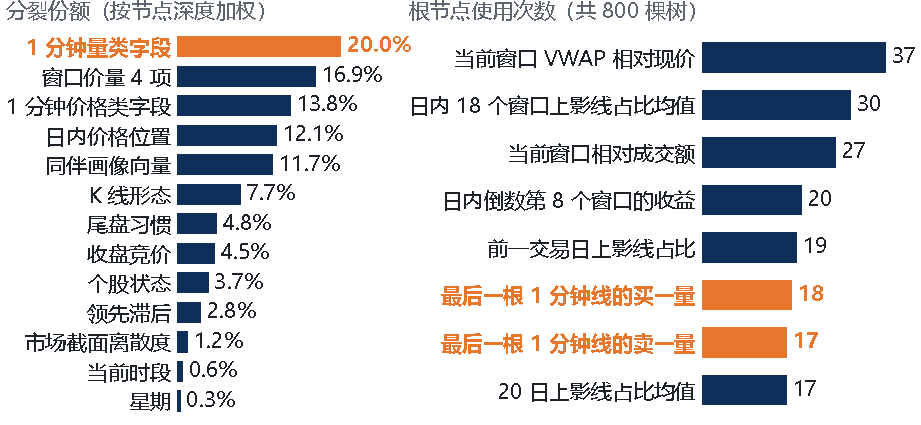
\includegraphics[width=\textwidth]{figures/fig_tree_splits_r.pdf}
\source{比赛平台分钟行情，团队计算}
\end{figure}

价格相对均价的位置是首要依据。标签度量的是窗口收盘价相对窗口均价的位置，梯度提升树子模型根节点最常用的特征为“当前窗口 VWAP 相对现价”（37 次）。当前价偏离窗口均价的程度，与下一窗口价格回到均价附近还是继续偏离直接相关。K 线形态提供同类信息：日内 18 个窗口上影线占比均值（30 次）、前一交易日上影线占比（19 次）与 20 日上影线占比均值（17 次）都在根节点常用特征之列，上影线较长对应盘中冲高回落时的抛压。

成交活跃度与一档挂单量是第二类依据。“当前窗口相对成交额”在根节点使用 27 次；按通道组深度加权，1 分钟量类字段的份额最高（20.0\%），其后是窗口价量 4 项（16.9\%）、1 分钟价格类字段（13.8\%）、日内价格位置（12.1\%）与同伴画像（11.7\%）；最后一根 1 分钟线的买一量、卖一量分别有 18 棵、17 棵树在根节点使用。神经网络方面，多任务头要求共享表示预测之后 30 分钟的已实现波动与成交量变化，这一辅助任务使 RankIC 在三个随机种子、两个年份上全部提高。分裂份额属于分裂次数类指标，不是增益重要性；梯度提升树在集成中占 1/7 的权重，这些统计不能外推为神经网络使用的信息。

\figref{fig:slot} 给出与最终模型同结构、只训练到 2022 年的留出验证模型在各截面的 RankIC。

\begin{figure}[htbp]
\caption{14:30 截面的 RankIC 约为其余时段均值的 1.6～1.8 倍，14:00 最弱（留出验证模型，2023–2024）}\label{fig:slot}
\centering
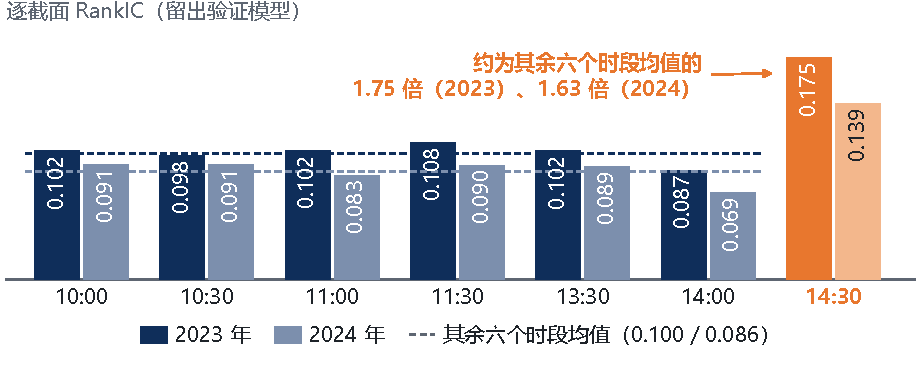
\includegraphics[width=\textwidth]{figures/fig_slot_ic_r.pdf}
\source{比赛平台分钟行情，团队本地评测}
\end{figure}

分时段看，14:30 截面最强，2023、2024 年 RankIC 分别为 0.175 与 0.139，是其余六个截面均值的 1.75 倍与 1.63 倍；四个半年里 14:30 都是其余时段均值的 1.4～1.9 倍，14:00 都最弱。14:30 的标签窗口跨过收盘集合竞价，将标签分解后，模型的预测能力集中在连续竞价段的漂移上：单模型对完整标签的 RankIC 为 0.156，对连续竞价段漂移为 0.135，对收盘竞价跳动只有 0.030。为加强收盘竞价部分做过两次尝试，都使 ICIR 下降，没有采用。

\figref{tab:ablation} 汇总单组件消融的结果，用来判断三个尺度与各组件之间的分工。

\begin{table}[htbp]
\caption{去掉单个组件后的四项指标（单随机种子，2023 年）}\label{tab:ablation}
\centering\tabsetup
\begin{tabular}{@{}lrrrr@{}}
\toprule
去掉的组件 & RankIC & ICIR & 压力稳定性 & 换手率\\
\midrule
对照（完整结构） & 0.1089 & 2.079 & 2.063 & 0.574\\
三个专家头的辅助监督 & 0.1078 & 2.077 & 2.039 & 0.580\\
同伴注意力（改为减截面平均） & 0.1098 & 2.068 & 2.021 & 0.580\\
日线尺度编码器 & 0.1072 & 2.116 & 2.063 & 0.589\\
日内尺度编码器 & 0.1042 & 2.132 & 2.023 & 0.586\\
多周期辅助目标 & 0.1119 & 2.139 & 2.075 & 0.654\\
\bottomrule
\end{tabular}
\source{比赛平台分钟行情，团队本地评测}
\end{table}

日内尺度贡献的 RankIC 最多，去掉后 RankIC 降低 0.0047，是所有消融项中降幅最大的一项。日线尺度主要起稳定作用：日线输入在同一交易日内几乎不变，去掉后换手率升高 0.015。同伴注意力改为减截面平均后压力稳定性降低 0.042；去掉三个专家头的辅助监督，RankIC 与压力稳定性都下降。多周期辅助目标以约 0.003 的 RankIC 换来 0.080 的换手率下降。去掉日内或日线尺度后 2023 年 ICIR 上升约 0.04～0.05，这一结果只有单随机种子、单一年份，没有在 2024 年复核，结构因此没有简化；差别小于随机种子噪声的项目都不作结论。

模型读取的信息与结构到此确定。每个截面独立预测，不加换手约束的单模型换手率偏高，第~\ref{sec:turn}~章讨论如何在训练中降低换手。

% ======================================================================
\section{在训练中控制换手}\label{sec:turn}

规则不允许推理时读取之前截面的输出，每个截面独立预测，不加换手约束的单模型本地换手率约 0.57。换手率是五项之一，输出平滑又被规则排除，我们用两项只在训练中起作用的设计控制换手。多周期辅助目标使预测偏向更持久的信号，单变量线上验证中换手率降低 0.046；多空组合换手正则项把同日相邻两个截面配成一组，只惩罚名单边界附近的进出，强度 0.1 时单模型公榜换手率降低 0.036，RankIC 只降低 0.0015。推理时每个截面仍然独立预测，两项设计都不改变推理路径。

\subsection{每个截面独立预测使换手偏高}\label{sec:turn-high}

没有输出平滑时，相邻两个截面的预测只通过输入的重叠部分产生联系，截面之间的小幅扰动会直接改变多空名单。不加换手正则项的单模型，留出验证设定下本地换手率为 0.573（2023 年）与 0.569（2024 年），单变量线上验证中公榜换手率为 0.551。

早期尝试的全局换手惩罚对全部股票相邻截面标准化得分之差的平方施加惩罚，在单变量线上验证中使换手率降低 0.10，但 RankIC 降低 0.006、多空组合夏普比率降低 4.8，因此被否决（第~\ref{sec:innov}~章）。它惩罚了评测不计入的变化：名单内部与中间股票的得分变动不影响换手率，却同样受到惩罚，模型为此损失了排序精度。

\subsection{多周期辅助目标偏向持久信号}\label{sec:multi}

多周期辅助目标包含在训练目标中（式~\eqref{eq:target}）：在当期标签的秩高斯目标上，加 0.5 倍“同一交易日之后 2 个截面标签之和”的秩高斯目标。它只改变训练目标，不改变推理，也不使用模型之前的输出。模型同时学习之后 30 分钟与之后 1 小时的相对表现。相邻两个截面的训练目标因此含有相同的标签分量：截面 $t$ 的辅助目标与截面 $t+1$ 的当期标签、辅助目标都有重叠，相邻截面之间的排序随之更连贯。

本地两年换手率降低 0.041～0.045，RankIC 提高 0.0004～0.0009；单变量线上验证中换手率降低 0.046，ICIR 提高 0.041。单组件消融中去掉这一目标，2023 年 RankIC 由 0.1089 升至 0.1119，换手率则由 0.574 升至 0.654。权重增至 1.0 时换手率再降约 0.04，但 RankIC 降低 0.006，未采用。

\subsection{多空组合换手正则项只作用于名单边界}\label{sec:legturn}

评测换手只计前、后 10\% 两端名单在同日相邻截面之间的进出，换手控制应当只作用于这一部分。训练时把同一交易日相邻的两个截面 $a$、$b$ 配成一个训练单元。融合头输出先对风格变量取残差并截面标准化，记为 $c$；$h_a$、$l_a$ 为截面 $a$ 上 $c$ 的第 90 与第 10 百分位。对两个截面都有的股票集合 $J$，定义多头、空头组合的软隶属度与正则项：
\begin{gather}
m^{+}_{a}(j)=\sigma\Big(\frac{c_a(j)-h_a}{\tau}\Big),\qquad m^{-}_{a}(j)=\sigma\Big(\frac{l_a-c_a(j)}{\tau}\Big),\qquad \tau=0.15,\label{eq:member}\\
L_{\text{turn}}(a,b)=\frac{1}{|J|}\sum_{j\in J}\Big[\big(m^{+}_{a}(j)-m^{+}_{b}(j)\big)^2+\big(m^{-}_{a}(j)-m^{-}_{b}(j)\big)^2\Big].\label{eq:legturn}
\end{gather}
总损失中取全部相邻截面对的平均，权重 0.1（式~\eqref{eq:total}）。\figref{fig:legturn} 说明这一项只惩罚名单边界附近进出的原因。

\begin{figure}[htbp]
\caption{多空组合换手正则项只惩罚名单边界附近的进出（示意，多头组合一侧）}\label{fig:legturn}
\centering
\begin{tikzpicture}[x=1cm,y=1cm]
  \draw[rgrey,line width=0.5pt,-{Stealth[length=1.6mm]}] (0,0)--(7.3,0);
  \draw[rgrey,line width=0.5pt,-{Stealth[length=1.6mm]}] (0,0)--(0,2.75);
  \draw[rgrey] (-0.08,2.2)--(0,2.2);
  \node[note,anchor=east] at (-0.1,0) {0};
  \node[note,anchor=east] at (-0.1,2.2) {1};
  \node[note,anchor=west] at (0.1,2.95) {多头隶属度};
  \node[note] at (3.85,-0.42) {残差标准化得分};
  \draw[rline,dashed,line width=0.6pt] (4.6,0)--(4.6,2.6);
  \node[note] at (4.6,2.9) {名单边界};
  \draw[rnavy,line width=0.9pt,domain=0.15:7.1,samples=90,smooth]
       plot (\x,{2.2/(1+exp(min(9,-(\x-4.6)/0.35)))});
  \node[note] at (1.6,0.68) {几乎无梯度};
  \node[note] at (6.55,1.55) {几乎无梯度};
  % A：名单内移动
  \fill[rgrey] (6.0,2.18) circle (2.2pt);
  \draw[rgrey,line width=0.8pt,fill=white] (6.9,2.2) circle (2.2pt);
  \draw[-{Stealth[length=1.6mm]},rgrey,line width=0.6pt] (6.1,2.42)--(6.8,2.42);
  \node[note] at (6.45,2.72) {A};
  % B：跨越边界
  \fill[raccent] (5.0,1.67) circle (2.2pt);
  \draw[raccent,line width=0.8pt,fill=white] (4.15,0.43) circle (2.2pt);
  \draw[-{Stealth[length=1.6mm]},raccent,line width=0.8pt] (4.92,1.5)--(4.25,0.6);
  \node[note,text=raccent] at (5.15,0.85) {B};
  % C：名单外移动
  \fill[rgrey] (1.0,0.03) circle (2.2pt);
  \draw[rgrey,line width=0.8pt,fill=white] (2.0,0.06) circle (2.2pt);
  \draw[-{Stealth[length=1.6mm]},rgrey,line width=0.6pt] (1.1,0.22)--(1.9,0.22);
  \node[note] at (1.5,-0.25) {C};
  \node[font=\sffamily\small,anchor=west,align=left] at (7.6,1.25) {%
    \renewcommand{\arraystretch}{1.6}%
    \begin{tabular}{@{}lll@{}}
    {\color{rgrey}A\quad 名单内移动} & {\color{rgrey}隶属度差约 0} & {\color{rgrey}不惩罚}\\
    {\color{raccent}B\quad 跨越名单边界} & {\color{raccent}隶属度差大} & {\color{raccent}惩罚}\\
    {\color{rgrey}C\quad 名单外移动} & {\color{rgrey}隶属度差约 0} & {\color{rgrey}不惩罚}
    \end{tabular}};
\end{tikzpicture}
\source{团队整理}
\end{figure}

sigmoid 函数只在名单边界附近有明显的斜率。图中实心点为前一截面，空心点为后一截面。名单内部的股票（A）与名单外的股票（C）在相邻截面之间移动时，隶属度几乎不变，正则项不产生梯度；跨越边界的股票（B）隶属度由接近 1 变为接近 0，受到惩罚。这与评测换手率的定义一致：只有进出名单的变化计入换手。推理时每个截面独立预测，不使用之前的输出，也不计算这一项。

相对只配对、不加正则项的对照，强度 0.1 使本地换手率降低 0.062，RankIC 两年分别降低 0.0016 与 0.0014。单变量线上验证中换手率降低 0.036，RankIC 降低 0.0015，ICIR 降低 0.030，压力稳定性与多空组合夏普比率的变化仅为 +0.004 与 −0.38。

\subsection{正则强度超过 0.1 后 ICIR 明显下降}\label{sec:strength}

正则强度 $\lambda$ 决定换手率与信号质量之间的取舍。\figref{fig:strength} 左栏为留出验证设定下单模型的本地换手率与 ICIR 随强度的变化，右栏为同一组强度的单变量线上验证。

\begin{figure}[htbp]
\caption{正则强度取 0.1 时只降换手，0.3 以上 ICIR 与压力稳定性明显下降（单模型，本地 2023–2024 与单变量线上验证）}\label{fig:strength}
\centering
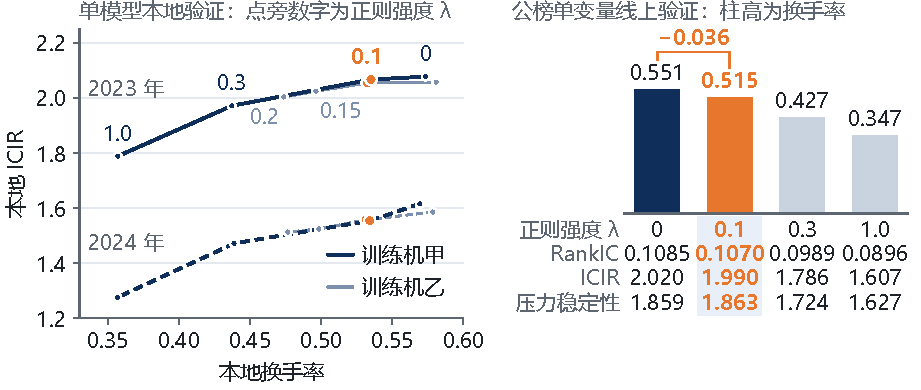
\includegraphics[width=\textwidth]{figures/fig_turnover_reg_r.pdf}
\source{比赛平台分钟行情，团队本地评测；比赛平台公榜，团队整理}
\end{figure}

强度由 0 增至 1.0，本地 2023 年换手率由 0.573 降至 0.357，ICIR 由 2.078 降至 1.789。公榜综合得分对 ICIR 与压力稳定性的敏感度高于换手率。单变量线上验证中，强度 0.1 时换手率降低 0.036、ICIR 只降低 0.030，压力稳定性由 1.859 变为 1.863；强度 0.3 时 ICIR 降至 1.786、压力稳定性降至 1.724，强度 1.0 时分别降至 1.607 与 1.627，换手率下降的收益不足以抵消这两项的损失，公榜得分随之下降。本地补测的 0.15 与 0.2 两档落在 0.1 与 0.3 两档之间；加入梯度提升树子模型之后，强度 0.15 相对 0.1 换手率再降 0.025，RankIC 却降低 0.0032、ICIR 降低 0.047、压力稳定性降低 0.032，同样不如 0.1。

\subsection{权重滑动平均降低随机种子差异}

训练时对网络参数做衰减系数 0.995 的指数滑动平均，即每步更新 $\bar\theta\leftarrow 0.995\,\bar\theta+0.005\,\theta$，推理加载平均后的参数 $\bar\theta$。同一配方两个随机种子的预测截面秩相关由 0.878 与 0.871 升至 0.941 与 0.934（2023 与 2024 年），单变量线上验证中换手率降低 0.016。权重滑动平均是训练时对参数的平均，与输出平滑无关：推理时每个截面独立做前向计算，不保存、不读取之前截面的输出。

单模型的换手控制止于强度 0.1，继续加强会损害 ICIR；进一步降低换手要依靠集成的构成（第~\ref{sec:ens}~章）。

% ======================================================================
\section{用信息不同的子模型组成集成}\label{sec:ens}

同一配方增加随机种子，子模型之间的预测相关仍在 0.93 左右，同配方子模型由 3 个增至 6 个，集成不再提升。我们改为加入信息或归纳偏置不同的子模型：一个读取三档盘口与委托笔数的梯度提升树，补充神经网络没有学到的挂单信息；两个只把序列编码器换成 GRU 的神经网络，用于降低换手。在留出验证模型上，加入梯度提升树使 2023 年 RankIC 提高 0.0028，再加入 2 个 GRU 使换手率两年都降低约 0.008，其余四项基本不变。

\subsection{7 个子模型等权排名平均}

\figref{fig:ens} 给出集成方式与子模型之间的截面秩相关。

\begin{figure}[htbp]
\caption{7 个子模型的集成方式与两两截面秩相关（相关系数取自留出验证模型，2024 年）}\label{fig:ens}
\centering
\begin{tikzpicture}[x=1cm,y=1cm]
  \tikzset{grp/.style={node,minimum width=3.4cm,minimum height=0.95cm}}
  \node[grp] (T) at (2.4,0) {4 个 Transformer\\族内相关 0.937};
  \node[grp] (G) at (6.6,0) {2 个 GRU\\族内相关 0.926};
  \node[key,minimum width=3.4cm,minimum height=0.95cm] (B) at (10.8,0) {1 个梯度提升树\\800 棵、深度 8};
  \draw[decorate,decoration={brace,amplitude=5pt},draw=rnavy,line width=0.6pt]
       ($(T.north west)+(0,0.12)$) -- ($(G.north east)+(0,0.12)$)
       node[midway,above=5pt,note] {两族之间 0.89～0.90};
  \draw[decorate,decoration={brace,amplitude=5pt},draw=rnavy,line width=0.6pt]
       ($(T.north west)+(0,0.95)$) -- ($(B.north east)+(0,0.95)$)
       node[midway,above=5pt,note] {梯度提升树与神经网络 0.75～0.76};
  \node[node,text width=11.6cm,minimum height=0.8cm] (W) at (6.6,-1.55) {每个子模型逐截面排名、减去 0.5，7 个子模型等权平均};
  \draw[flow] (T.south)--(T.south |- W.north);
  \draw[flow] (G.south)--(G.south |- W.north);
  \draw[flow] (B.south)--(B.south |- W.north);
  \node[node] (n1) at (6.6,-3.0) {4 个风格特征\\中性化};
  \node[node] (n2) at (9.6,-3.0) {09:30 截面\\输出 0};
  \node[key] (n3) at (12.4,-3.0) {最终输出};
  \draw[flow] (W.south -| n1)--(n1);
  \draw[flow] (n1)--(n2);
  \draw[flow] (n2)--(n3);
\end{tikzpicture}
\source{比赛平台分钟行情，团队计算}
\end{figure}

最终模型包括 4 个 Transformer（随机种子 42～45，每个 201,830 个参数）、2 个 GRU（随机种子 46、47，每个 167,782 个参数）与 1 个梯度提升树（800 棵、深度 8），神经网络合计 1,142,884 个参数。每个子模型逐截面排名后减 0.5，7 个子模型等权平均（式~\eqref{eq:ens}），再做风格中性化。子模型之间相关很高，学习集成权重难以稳定优于等权，权重扫描只针对梯度提升树进行。同族不同随机种子的子模型相关在 0.93 左右，GRU 与 Transformer 为 0.89～0.90，梯度提升树与神经网络为 0.75～0.76，模型族不同的子模型之间预测差异更大。

\subsection{梯度提升树补充挂单信息}

神经网络预测与每笔挂单规模类信号的相关只有 0.03～0.07，控制神经网络预测之后，这些信号仍有约 0.01 的偏 RankIC。把同样的三档字段与委托笔数输入 Transformer，它也未能学到这部分信息。挂单信息需要另一类模型读取。

梯度提升树子模型使用 800 棵树、深度 8、学习率 0.03、行抽样 50\%、列抽样 70\%、叶子最少 1000 个样本、L2 正则 1、64 箱分箱，输入为第~\ref{sec:input}~节的 1055 个池化特征。平台默认环境没有 LightGBM 与 sklearn，梯度提升树以 PyTorch 自行实现的直方图算法训练。训练目标与神经网络相同；改用同一目标之后，树进入集成的换手代价减半。

梯度提升树单独预测的效果弱于神经网络，换手更高（单独换手率约 0.60，神经网络单个子模型约 0.53），与神经网络的截面秩相关约 0.76。树能否带来增量取决于输入的信息：加特征、加深、增加树的数量都没有提高集成表现，换成三档全字段与委托笔数之后，四项第一次同时提高。同一时点比较中，加入树使公榜 RankIC 提高 0.0015、压力稳定性提高 0.007，换手率升高 0.003。

\subsection{GRU 子模型只降低换手，其余四项不变}\label{sec:gru}

\figref{fig:chain} 给出留出验证模型逐步加入各组件的增量：依次加入多空组合换手正则项、梯度提升树子模型与 2 个 GRU 子模型，最下一行是不加正则项时加入梯度提升树的对照。

\begin{figure}[htbp]
\caption{正则项降低换手，梯度提升树弥补 RankIC，GRU 子模型再降换手率 0.008（留出验证模型，2023–2024）}\label{fig:chain}
\centering
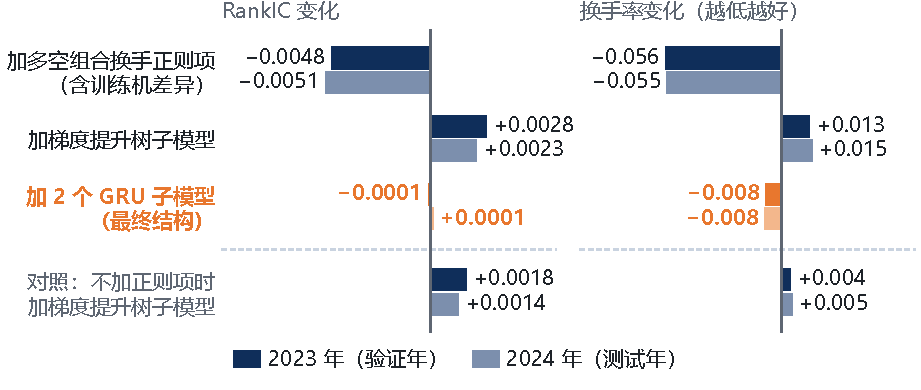
\includegraphics[width=\textwidth]{figures/fig_increment_chain_r.pdf}
\source{比赛平台分钟行情，团队本地评测}
\end{figure}

正则项使换手率降低约 0.056。这一步前后的 Transformer 子模型分别在两台训练机上训练，RankIC 的差值含有训练机不同带来的约 0.001～0.002 的差异；后两步沿用同一组 Transformer 子模型，不受这一影响。加入梯度提升树之后 RankIC 得到恢复，2023 年由 0.1079 升至 0.1107，换手率升高 0.013～0.015；同一操作在不加正则项时只带来 0.0018 与 0.0014 的 RankIC 提高。最后加入 2 个 GRU 子模型，换手率两年都降低 0.008，RankIC 的变化不超过 0.0001。\figref{fig:gru} 给出各项指标随 GRU 子模型个数的变化。

\begin{figure}[htbp]
\caption{换手率随 GRU 子模型个数单调下降，ICIR 变化不超过 1\%，最终结构取 2 个（留出验证模型，2023–2024）}\label{fig:gru}
\centering
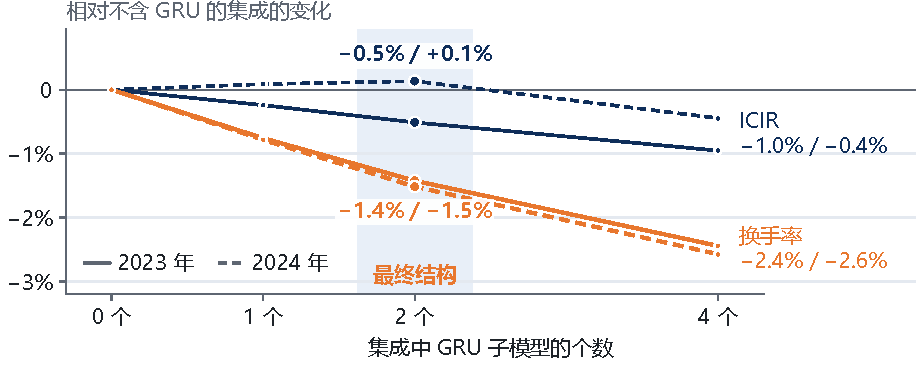
\includegraphics[width=\textwidth]{figures/fig_gru_count_r.pdf}
\source{比赛平台分钟行情，团队本地评测}
\end{figure}

换手率随 GRU 子模型个数单调下降，在两年、四种个数设置下方向一致：2023 年由 0.5421 依次降至 0.5380、0.5344 与 0.5288。其余四项在 0～2 个之间几乎不变，RankIC 的变化在 ±0.0001 以内；增至 4 个时 ICIR 开始下降（2023 年 2.048，2024 年 1.574）。GRU 单个子模型换手率的随机种子标准差约为 0.0033～0.0035，2 个 GRU 带来的 −0.008 是它的两倍以上，并且随个数单调变化。

\subsection{集成增益取决于信息差异与子模型强度}

集成的增益来自子模型所用信息或归纳偏置的差异，与子模型的个数关系不大：两种训练方式各 3 个子模型混合成 6 个，两年 RankIC 提高 0.002，而同配方的 6 个子模型不优于 3 个。相关更低也不一定更好：只读取盘口细节的梯度提升树与 Transformer 的相关只有 0.51，加入集成后 RankIC 提高 0.0009 与 0.0006，换手率却升高 0.019 与 0.020，净效果约为 0，没有采用。进入集成的子模型既要带来不同的信息，也要足够强、不推高换手。

第~\ref{sec:align}～\ref{sec:ens}~章的改动都依据 2023、2024 年的本地结果选定，第~\ref{sec:valid}~章检验它们在公榜与私榜上是否成立。

% ======================================================================
\section{验证流程与私榜作品选择}\label{sec:valid}

端到端模型的每项改动都要重新训练，同一配方换随机种子的差异与许多改动的增量处于同一量级。我们用三级验证流程筛选改动：留出验证单模型、单变量线上验证、全量训练。事后统计 21 组本地与公榜的配对，本地 RankIC 增量不低于 0.002 的 11 组公榜方向全部一致。与最终模型同结构、只训练到 2022 年的留出验证模型在 2023、2024 年的 RankIC 为 0.1106 与 0.0933；私榜四项较公榜回落 20\%～23\%，逐截面 RankIC 标准差与换手率基本不变。

\subsection{三级验证流程}\label{sec:gate}

改动先在留出验证设定下用单模型评估，两年分别判断增量是否超过随机种子噪声；再做单变量线上验证；两级都通过并满足全量训练准入标准，才训练全部 7 个子模型。\figref{fig:gate} 给出这一流程。

\begin{figure}[htbp]
\caption{改动从提出到全量训练的三级验证流程}\label{fig:gate}
\centering
\begin{tikzpicture}[x=1cm,y=1cm,node distance=7mm]
  \node[node,minimum height=0.95cm] (v1) at (1.9,0) {留出验证单模型\\2020–2022 年训练};
  \node[node,minimum height=0.95cm,right=of v1] (v2) {单变量线上验证\\公榜同一时点比较};
  \node[node,minimum height=0.95cm,right=of v2] (v3) {全量训练\\准入标准};
  \node[key,minimum height=0.95cm,right=of v3] (v4) {全量训练\\7 个子模型};
  \draw[flow] (v1)--(v2);
  \draw[flow] (v2)--(v3);
  \draw[flow] (v3)--(v4);
  \node[note,above=1.5mm of v1] {至少 223 个训练};
  \node[note,above=1.5mm of v2] {38 个有公榜结果的提交};
  \node[note,above=1.5mm of v4] {39 次全量训练};
  \node[note] (s1) at ($(v1.south)+(0,-1.0)$) {停止};
  \node[note] (s3) at ($(v3.south)+(0,-1.0)$) {停止};
  \draw[flow,draw=rline] (v1.south)--(s1.north);
  \draw[flow,draw=rline] (v3.south)--(s3.north);
  \node[soft,dashed] (ex) at ($(v2.south)+(0,-1.15)$) {全天 5 分钟片段\\本地为正，公榜 RankIC −0.0033};
  \draw[flow,draw=rline] (v2.south)--(ex.north);
\end{tikzpicture}
\source{团队整理}
\end{figure}

全量训练准入标准规定了五项增量的阈值：RankIC ≥ +0.005、ICIR ≥ +0.08、压力稳定性 ≥ +0.05、多空组合夏普比率 ≥ +1.5、换手率 ≤ +0.01。研究期间共有至少 223 个留出验证训练、38 个有公榜结果的端到端提交、39 次全量训练。流程也出现过未被遵守的情况：强度 0.3 的单变量线上验证结果返回之前，曾提前安排一次全量训练，团队成员发现后予以取消；该强度随后返回的 ICIR 只有 1.786。

\subsection{超过噪声的本地增量在公榜重现}\label{sec:transfer}

\figref{fig:transfer} 对比 21 组改动的本地增量与公榜增量：左栏为 RankIC 增量的散点，右栏为方向一致的计数。

\begin{figure}[htbp]
\caption{本地 RankIC 增量不低于 0.002 的 11 组改动，公榜方向全部一致（21 组配对）}\label{fig:transfer}
\centering
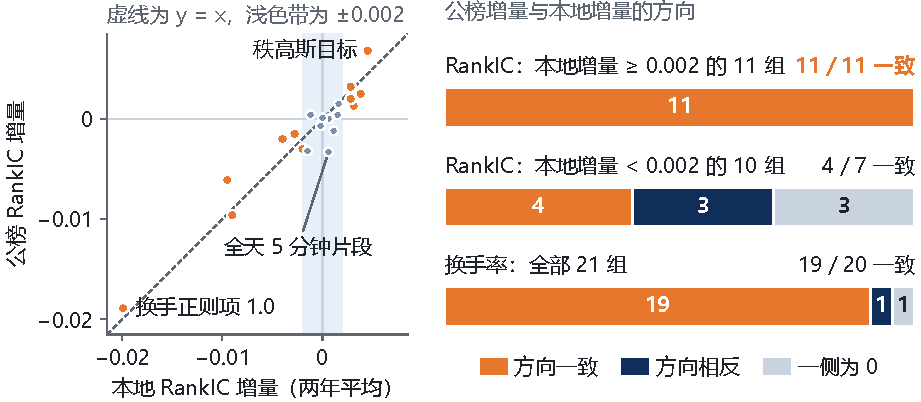
\includegraphics[width=\textwidth]{figures/fig_local_public_r.pdf}
\source{比赛平台公榜，团队整理；比赛平台分钟行情，团队本地评测}
\end{figure}

换手率的一致性最高：方向 19／20 一致，本地增量与公榜增量的相关为 0.986。RankIC 方向 15／18 一致，相关 0.953；ICIR 为 16／21，相关 0.899。按本地 RankIC 增量的大小分组，绝对值不低于 0.002 的 11 组公榜方向全部一致；小于 0.002 的 10 组只有 4 组同向、3 组反向、3 组一侧为 0。0.002 约为 1.5 个单随机种子标准差，增量低于这一水平的改动不作为采纳依据。

未能在公榜重现的改动集中在两类：日内细节类输入（如全天 5 分钟片段）与中间时刻样本（训练时在相邻评测截面之间加入的时点），它们在本地为正，在公榜上没有增量或方向相反。19 个单变量线上验证的公榜 RankIC 与本地 2023 年 RankIC 之比落在 0.97～1.06，平均 1.00，单模型的本地水平可以直接对应公榜水平。

\subsection{留出年份与半年度稳定性}

最终模型训练到 2024 年底，本身没有本地样本外指标；样本外证据来自与最终模型同结构、只训练到 2022 年的留出验证模型。两者的 GRU 随机种子与 Transformer 的训练机不同，同一配方换训练机的 RankIC 差约 0.001～0.002。\figref{tab:results} 汇总留出验证模型两年与最终模型公榜、私榜的五项。

\begin{table}[htbp]
\caption{留出验证模型 2023、2024 年与最终模型公榜、私榜的五项指标}\label{tab:results}
\centering\tabsetup
\begin{tabular}{@{}lrrrr@{}}
\toprule
指标 & 留出验证 2023 年 & 留出验证 2024 年 & 最终模型公榜 & 最终模型私榜\\
\midrule
RankIC & 0.1106 & 0.0933 & 0.1143 & 0.0888\\
ICIR & 2.057 & 1.583 & 2.019 & 1.564\\
多空组合夏普比率 & 64.01 & 47.55 & 56.33 & 44.98\\
压力稳定性 & 2.028 & 1.402 & 1.900 & 1.460\\
换手率 & 0.534 & 0.534 & 0.508 & 0.500\\
\bottomrule
\end{tabular}
\source{比赛平台分钟行情，团队本地评测；比赛平台公榜／私榜，团队整理}
\end{table}

最终模型位列公榜第四、私榜第六。私榜五项由平台按提交的训练脚本从零重训的模型评出（第~\ref{sec:limit-ch}~章）。表中的多空组合夏普比率衡量信号对多空两端的区分程度，不含交易成本，不等于可实现收益。

按半年度拆分（附录~\ref{app:half}），留出验证模型四个半年的 RankIC 为 0.1166、0.1049、0.0899、0.0964。各项最大值与最小值之比为 RankIC 1.30、ICIR 1.33、多空组合夏普比率 1.46、压力稳定性 1.53、换手率 1.02。换手率最稳定，其余四项随行情环境同涨同跌，没有任何一个半年出现信号失效。加入 2 个 GRU 的增量在四个半年方向一致，换手率降低 0.0074～0.0088，压力稳定性提高 0.002～0.006。

以 242 个交易日每天一个观测计算，2023 年 ICIR 对应的 $t$ 统计量约为 32.0，2024 年约为 24.6。这一计算未处理跨日自相关；对端到端模型而言，更主要的不确定性来自重新训练的随机性。

\subsection{私榜回落来自信号水平，波动未变}

按\figref{tab:results} 的五项计算，私榜与公榜之比为 RankIC 0.777、ICIR 0.775、多空组合夏普比率 0.798、压力稳定性 0.769、换手率 0.984。逐截面 RankIC 的标准差公榜为 0.0566、私榜为 0.0568，压力稳定性与 ICIR 之比公榜为 0.941、私榜为 0.934。回落的是信号水平，波动没有变化。

本地相邻两年有同样幅度的回落：留出验证模型 2024 年的 ICIR 是 2023 年的 0.770；私榜相对本地 2024 年，RankIC 之比为 0.952、ICIR 之比为 0.988。因子赛道同期的私榜与公榜之比为 RankIC 0.768、ICIR 0.754，两个赛道的模型输出与因子值互相隔离、构造方法不同，回落幅度却相近，一种解释是私榜区间整体信号较弱。这一旁证有局限：两个赛道预测同一标签、研究思路相互借鉴，不是独立样本。

\subsection{私榜作品的选择依据}

私榜每队只能选一个作品，我们选择在每个半年都成立、增量没有以其他指标为代价的版本。最终模型相对加入 2 个 GRU 之前的集成，只有换手率下降、其余四项持平，这一点在本地两年、四个半年和公榜同一时点比较三方面一致。含 4 个 GRU 的版本换手率再降约 0.0055，但四个半年 RankIC 降低 0.0002～0.0003、ICIR 降低 0.005～0.013，团队成员担心对公榜过拟合，没有提交。

第~\ref{sec:align}～\ref{sec:valid}~章的设计中有四处与常规做法不同，第~\ref{sec:innov}~章逐一比较，并说明各自成立的条件。

% ======================================================================
\section{与常规做法的四处差别}\label{sec:innov}

端到端选股模型的常规做法包括回归收益率、用官方风格暴露中性化、在推理端平滑输出、以同一配方的多个随机种子集成、依据本地回测或公榜得分选择方案。本赛道的两条规则与评测口径使这些做法部分失效或不可用，最终模型与常规做法的差别集中在四处（\figref{tab:innov}）。

\begin{table}[htbp]
\caption{与常规做法相比的四处差别（概要）}\label{tab:innov}
\centering\tabsetup
\begin{tabularx}{\textwidth}{@{}p{4.2em}>{\raggedright\arraybackslash}X>{\raggedright\arraybackslash}X>{\raggedright\arraybackslash}X@{}}
\toprule
设计 & 常规做法 & 我们的做法 & 适用条件\\
\midrule
换手控制 & 推理端平滑输出；训练中惩罚全部股票的得分变化 & 只惩罚同日相邻截面跨越多空名单边界的进出 & 评测换手只计多空两端；强度不宜超过 0.1\\
训练目标 & 回归收益率或其标准化值；用官方风格暴露中性化 & 秩高斯目标，对行情代理与聚类行业取残差 & 评测为残差上的秩相关；线上不提供风格暴露\\
集成构成 & 同一配方的多个随机种子 & 加入读取三档盘口的梯度提升树与 GRU 子模型 & 子模型足够强且不推高换手\\
改动筛选 & 仅凭本地回测，或仅凭公榜得分 & 增量超过随机种子噪声，再经单变量线上验证 & 只能识别效应较大的改动\\
\bottomrule
\end{tabularx}
\source{团队整理}
\end{table}

\subsection{只惩罚名单边界进出的换手正则项}

推理端的输出平滑与换手缓冲带被规则禁止，训练中可用的常规做法是全局换手惩罚，即惩罚全部股票相邻截面得分之差的平方。多空组合换手正则项（第~\ref{sec:legturn}~节）只惩罚多空名单隶属度的变化，梯度集中在名单边界附近。

两种做法在单变量线上验证中的代价相差很大：全局换手惩罚使换手率降低 0.10，但 RankIC 降低 0.006、多空组合夏普比率降低 4.8，公榜得分随之下降；多空组合换手正则项在强度 0.1 时使换手率降低 0.036，RankIC 只降低 0.0015、多空组合夏普比率只降低 0.38，公榜得分随之上升。本地留出验证中，全局换手惩罚每损失 0.001 的 RankIC 只换来 0.013 的换手率下降，正则项以两年 0.0016 与 0.0014 的 RankIC 损失换来 0.062 的换手率下降。全局换手惩罚的大部分约束作用于评测不计入的排序变化。

这一设计成立有三个条件：评测换手只计多空两端与同日相邻截面，若评测改为全截面的排序稳定性，它不再有优势；强度有上限，强度 0.3 起 ICIR 降低约 0.2；训练批次需要由同日相邻截面配对组成。

\subsection{不依赖官方风格暴露的目标对齐}

常规做法回归收益率或其截面标准化值，剔除风格时直接使用官方风格暴露。最终模型的训练目标只保留排序，并对行情代理风格因子、规模平方项与聚类行业取残差（第~\ref{sec:rg}～\ref{sec:loss}~节）；整个过程只使用原始行情，私榜重训时同样可以运行。

秩高斯目标相对截面标准化目标，使单模型两年 RankIC 提高 0.0042 与 0.0039，单变量线上验证中 ICIR 提高 0.193、压力稳定性提高 0.204。中性化方面，训练时直接使用官方风格暴露两年都更差：2023 年 RankIC 0.1079 对 0.1089，2024 年 0.0902 对 0.0926。

这一设计以评测在残差上计算秩相关、线上不提供风格暴露为前提。行情代理对量价类风格的替代程度较高（平均截面 $R^2$ 为 0.64～0.79），对规模与财务类风格较低（SIZE 0.44，GROWTH 0.17）；单个子模型的输出中仍有约 21\%（2023 年）与 22\%（2024 年）的截面方差可由官方风格与行业解释。评测中财务类风格比重越大，对齐越不充分。

\subsection{以不同模型族的子模型补充信息、降低换手}

同一配方、不同随机种子的子模型使用的信息相同，预测相关在 0.93 左右，子模型由 3 个增至 6 个，集成不再提升。最终模型改为加入梯度提升树与 GRU 两类子模型，前者补充挂单信息，后者降低换手（第~\ref{sec:ens}~章）。

在留出验证模型上，加入梯度提升树使 2023 年 RankIC 提高 0.0028；再加入 2 个 GRU 使换手率两年都降低约 0.008，其余四项的变化在随机种子噪声以内（第~\ref{sec:gru}~节）。

这一做法要求新加入的子模型带来不同的信息，同时足够强、不推高换手。只读取盘口细节的梯度提升树与 Transformer 相关只有 0.51，加入后换手率升高 0.019 与 0.020，净效果约为 0；GRU 增至 4 个时 ICIR 开始下降。

\subsection{以随机种子噪声与线上验证两级筛选改动}

仅凭本地回测容易把单随机种子的噪声当作增量，仅凭公榜得分则带有选择偏差，不同日期的得分也不可比。三级验证流程（第~\ref{sec:gate}~节）要求本地增量两年都超过随机种子噪声，并在单变量线上验证中与对照在同一时点比较。

事后统计的 21 组配对中，本地 RankIC 增量不低于 0.002（约 1.5 个单随机种子标准差）的改动公榜方向全部一致，低于 0.002 的 10 组只有 4 组同向（第~\ref{sec:transfer}~节）。全天 5 分钟片段在本地两年为正，未通过第二级验证，没有进入全量训练。

这一流程只能可靠地识别效应较大的改动，增量小于随机种子噪声的改动无法判断。单变量线上验证本身也带有选择偏差；2023、2024 年都参与过方案选择，没有参与选择的只有私榜。最终模型最后一步改动的增量是换手率下降，换手率也是本地与公榜一致性最高的指标。

这四处差别只在本文的数据与规则下检验过，检验的边界在第~\ref{sec:limit-ch}~章说明。

% ======================================================================
\section{研究方法与结论边界}\label{sec:limit-ch}

评价上述结论还需要说明三个问题：工作如何在团队成员与 AI 编码代理之间分工，推理是否用到未来信息，训练能否复现。最终模型通过了截断检测，同一份脚本可以从零训练出统计上等价的模型；结论的主要局限在于私榜只有一个区间、最终模型本身没有本地样本外指标、换手率仍约 0.50。

\subsection{团队成员与 AI 编码代理的分工}

端到端赛道的代码、实验、分析、打包与记录几乎全部由 AI 编码代理（Claude Code）完成：涉及端到端目录的 205 个代码提交中，204 个由它提交，唯一的例外是仓库初始化。团队成员负责确定评价标准与研究方向、判断合规性、向平台上传作品并转达公榜结果、决定每轮改动是否采用与是否提交，以及选择私榜作品；AI 编码代理不接触比赛平台。被团队成员否决的 AI 产出包括输出平滑、以因子为基础的路线、提前安排的全量训练与含 4 个 GRU 的版本，详细分工见单独提交的 AI 工具使用说明。

\subsection{截断检测与可复现性}

\begin{figure}[htbp]
\caption{截断检测的做法（2024 年 3 月 4 日起，截断于 3 月 6 日 10:30 与 14:30）}\label{fig:leak}
\centering
\begin{tikzpicture}[x=1cm,y=1cm]
  \draw[rgrey,line width=0.5pt] (0,0)--(8.0,0);
  \foreach \d in {0,1,2,3}{
    \draw[rgrey] (\d*2.0,-0.12)--(\d*2.0,0.12);
    \foreach \s in {0,...,7}{\draw[rline] (\d*2.0+\s*0.25+0.125,0)--(\d*2.0+\s*0.25+0.125,0.08);}
  }
  \draw[rgrey] (8.0,-0.12)--(8.0,0.12);
  \foreach \d/\t in {0/3 月 4 日,1/3 月 5 日,2/3 月 6 日,3/3 月 7 日}{\node[note] at (\d*2.0+1.0,-0.38) {\t};}
  \draw[raccent,line width=1.1pt] (4.625,-0.05)--(4.625,2.05);
  \draw[raccent,line width=1.1pt] (5.875,-0.05)--(5.875,2.05);
  \node[note,text=raccent] at (4.625,2.3) {10:30};
  \node[note,text=raccent] at (5.875,2.3) {14:30};
  \draw[rnavy,line width=0.6pt,rounded corners=1.5pt] (0,1.3) rectangle (8.0,1.75);
  \node[font=\sffamily\small] at (2.3,1.525) {全量数据};
  \draw[rnavy,line width=0.6pt,rounded corners=1.5pt] (0,0.5) rectangle (5.875,0.95);
  \node[font=\sffamily\small] at (2.3,0.725) {截断数据};
  \draw[rline,dashed,line width=0.6pt,rounded corners=1.5pt] (5.875,0.5) rectangle (8.0,0.95);
  \node[note] at (6.94,0.725) {删除};
  \node[node] (m) at (10.2,1.12) {同一打包模型\\完整推理路径};
  \draw[flow] (8.05,1.525)--(m.west |- 0,1.45);
  \draw[flow] (8.05,0.725)--(m.west |- 0,0.8);
  \node[key] (k) at (13.45,1.12) {逐行比较预测\\差值超过 $10^{-6}$：0 行};
  \draw[flow] (m)--(k);
  \node[note] at (13.45,0.0) {19,000 行与 24,000 行};
\end{tikzpicture}
\source{团队整理}
\end{figure}

推理是否用到截面之后的信息，由截断检测检验，做法见\figref{fig:leak}。同一个打包模型做两次推理，一次读取全量数据，一次只读取截断时刻及之前的数据，7 个子模型、截面排名、中性化与 09:30 输出 0 原样运行。截断时刻及之前的 19,000 行与 24,000 行预测中，差值超过 $10^{-6}$ 的行数为 0；任何环节用到截断之后的数据，包括经截面排名、同伴注意力或中性化间接用到，两次预测都会不同。代码中另设有特征时点断言。检测的局限在于只抽取了 4 个交易日、2 个截断时刻，使用的是本地数据后端，不覆盖平台 SQL 本身。

本文所说的可复现，是指同一份代码、配置与随机种子能从零训练出统计上等价的模型；浮点运算的非确定性使权重不能逐位相同，同一配方换训练机的 RankIC 差约 0.001～0.002。私榜成绩来自平台按提交的训练脚本从零重训的模型，这说明训练流程在平台上可以复现，成绩不依赖本地训练得到的权重。

\subsection{局限与风险提示}\label{sec:limits}

\figref{tab:limits} 列出主要局限、受影响的结论以及已做和未做的检验。

\begin{table}[htbp]
\caption{局限、影响的结论与已做的检验}\label{tab:limits}
\centering\tabsetup
\begin{tabularx}{\textwidth}{@{}>{\raggedright\arraybackslash\hsize=1.05\hsize}X>{\raggedright\arraybackslash\hsize=0.8\hsize}X>{\raggedright\arraybackslash\hsize=1.15\hsize}X@{}}
\toprule
局限 & 影响的结论 & 已做或未做的检验\\
\midrule
私榜只有一个区间，日期未公布 & 公榜到私榜回落 20\%～23\% 的原因 & 本地相邻两年有同幅回落；行情环境与过拟合无法严格区分\\
最终模型没有本地样本外指标 & 第~\ref{sec:valid}~章的样本外数字 & 以同结构的留出验证模型代替；两者随机种子与训练机不同\\
换手率仍约 0.50（公榜 0.508，私榜 0.500） & 换手控制的效果 & 正则强度 0.3 以上 ICIR 与压力稳定性明显下降\\
神经网络未做逐通道归因 & 第~\ref{sec:behavior}~节的机制解释 & 只有组件消融与树的分裂统计；积分梯度、SHAP、置换重要性均未做\\
约五分之一的输出方差仍可由风格与行业解释 & 训练目标的中性化程度 & 单模型诊断为 21\%／22\%；行情代理对规模与财务类风格覆盖不全\\
未做正式显著性检验与含成本回测 & 多空组合夏普比率的含义 & 只给出未处理自相关的 $t$ 统计量；未计交易成本\\
\bottomrule
\end{tabularx}
\source{团队整理}
\end{table}

风险提示有三条：收盘集合竞价制度或盘口数据口径变化时，最先受影响的是 14:30 截面与梯度提升树子模型的挂单特征；同一配方重新训练，RankIC 约有 0.001～0.002 的差异；多空组合夏普比率不含交易成本，A 股空头端还受融券约束。

% ======================================================================
\newpage
\appendix
\ctexset{section={number=\Alph{section},
  numberformat={\color{white}\colorbox{rnavy}{\makebox[1.1em]{\Alph{section}}}}}}

\section{训练设置与训练轮数}\label{app:train}

\figref{tab:train} 列出神经网络子模型的训练设置与取值依据，梯度提升树子模型的设置见第~\ref{sec:ens}~章。

\begin{table}[htbp]
\caption{神经网络子模型的训练设置}\label{tab:train}
\centering\tabsetup
\begin{tabularx}{\textwidth}{@{}p{5.5em}>{\raggedright\arraybackslash}X>{\raggedright\arraybackslash}X@{}}
\toprule
参数 & 取值 & 依据\\
\midrule
训练区间 & 2020 年 1 月 1 日至 2024 年 12 月 31 日，固定在脚本中 & 私榜阶段平台从零重训\\
训练样本 & 8,461,813 个股票—截面样本，09:30 截面不参与，每个截面约 1,000 只股票 & 09:30 截面输出 0，不计分\\
优化器 & Adam，学习率 0.001 常数，梯度范数裁剪 1.0 & 学习率 0.0005、0.002 不优于现值；余弦衰减使 RankIC 降低 0.002～0.003\\
训练轮数 & 6 轮，不按验证集早停 & 相对 4 轮，三个随机种子两年换手率降低 0.014～0.015、RankIC 提高 0.0007～0.0008\\
批大小 & 每批 2 个配对训练单元（最多 4 个截面） & 每批 8 个截面不优于现值\\
dropout & 0.1 & —\\
权重滑动平均 & 衰减系数 0.995 & 随机种子间预测相关由 0.878 升至 0.941\\
损失权重 & 多空组合换手正则项 0.1（$\tau=0.15$），多任务头 0.5，多周期辅助目标 0.5 & 第~\ref{sec:strength}~节；多任务头与多周期目标取 1.0 均不如 0.5\\
随机种子 & 子模型 $k$ 用 $42+k$；打乱顺序、标准化统计量抽样、聚类、树的行列抽样全部固定 & 私榜重训可得到统计上等价的模型\\
\bottomrule
\end{tabularx}
\source{团队整理}
\end{table}

\figref{fig:epochs} 为单模型 8 轮训练的验证曲线（2020–2022 年训练，2023 年验证）。RankIC 在第 6 轮最高（0.1074），换手率在第 6 轮最低（0.573）；ICIR 在第 3 轮最高（2.128），第 6 轮为 2.091。第 8 轮 RankIC 回落至 0.1060，ICIR 回落至 2.068。最终模型固定训练 6 轮。

\begin{figure}[htbp]
\caption{验证年 RankIC 在第 6 轮最高，换手率在第 6 轮最低（单模型，单随机种子，验证年 2023）}\label{fig:epochs}
\centering
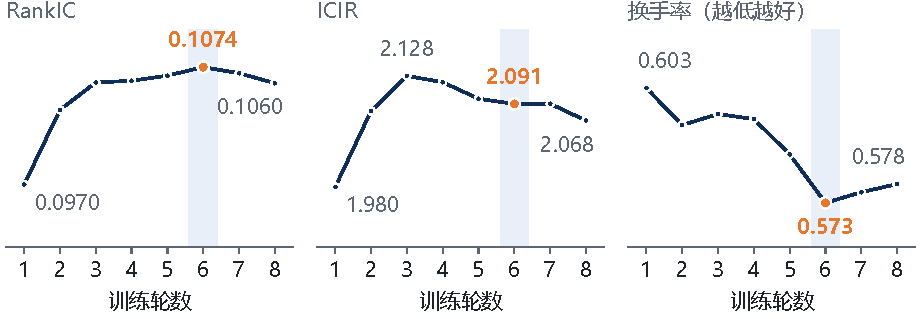
\includegraphics[width=\textwidth]{figures/fig_epochs_r.pdf}
\source{比赛平台分钟行情，团队本地评测}
\end{figure}

\section{未保留的方案}\label{app:rejected}

\figref{tab:rejected} 列出在本地或公榜验证中被否决的主要方案。

\begin{table}[htbp]
\caption{未保留的方案及其验证结果}\label{tab:rejected}
\centering\tabsetup
\begin{tabularx}{\textwidth}{@{}>{\raggedright\arraybackslash\hsize=1.0\hsize}X>{\raggedright\arraybackslash\hsize=1.0\hsize}X@{}}
\toprule
方案 & 验证结果\\
\midrule
隐层宽度加到 128 & 两年 RankIC 降低 0.0015 与 0.0021，ICIR 降低 0.058\\
1 分钟编码器加深到 3 层、4 层 & 换随机种子后与 2 层持平\\
截面 Transformer、注意力池化、跨尺度注意力、市场门控、同时段序列、推理时混入日线编码器输出 & 本地留出验证未通过\\
全天 5 分钟片段输入 & 本地两年为正；单变量线上验证 RankIC 降低 0.0033\\
全局换手惩罚 & 单变量线上验证换手率 −0.10，但 RankIC −0.006、多空组合夏普比率 −4.8\\
多周期辅助目标权重 1.0 & 换手率再降约 0.04，RankIC 降低 0.006\\
加强收盘竞价的两次尝试 & ICIR 下降\\
ICIR 稳定性项、尾部加权、列表式排序损失、SAM、离散度加权、按年或按时刻加权、按日抽样、两阶段残差提升、日线锚 & 本地留出验证否决\\
只读取盘口细节的梯度提升树子模型 & RankIC 提高 0.0009 与 0.0006，换手率升高 0.019 与 0.020，净效果约为 0\\
4 个 GRU 子模型 & 换手率再降约 0.0055，四个半年 ICIR 降低 0.005～0.013\\
推理端输出平滑 & 规则禁止，规则公布当天撤回并删除代码\\
\bottomrule
\end{tabularx}
\source{比赛平台分钟行情，团队本地评测；比赛平台公榜，团队整理}
\end{table}

\section{全部增量与证据}\label{app:increments}

\figref{tab:increments} 按加入顺序列出最终模型保留的全部改动。本地证据来自留出验证设定，公榜证据为单变量线上验证或同一时点比较。

\begin{table}[htbp]
\caption{最终模型保留的改动、本地证据与公榜证据}\label{tab:increments}
\centering\tabsetup
\begin{tabularx}{\textwidth}{@{}>{\raggedright\arraybackslash\hsize=0.7\hsize}X>{\raggedright\arraybackslash\hsize=1.2\hsize}X>{\raggedright\arraybackslash\hsize=1.1\hsize}X@{}}
\toprule
改动 & 本地证据 & 公榜证据\\
\midrule
09:30 截面输出 0、训练改用行情代理与聚类行业中性化、推理端中性化 & 09:30 输出 0 单项：两年五项全部改善，换手率 −0.035，RankIC +0.003～+0.005 & 三项合计，同一时点比较：压力稳定性 +0.16、多空组合夏普比率 +7.3、ICIR +0.065、换手率 −0.021、RankIC +0.0055\\
多周期辅助目标 & 换手率 −0.041～−0.045，RankIC +0.0004～+0.0009 & 换手率 −0.046，ICIR +0.041\\
融合头 & 2023 年 RankIC +0.0046、ICIR +0.145、压力稳定性 +0.130；2024 年 RankIC +0.0044、ICIR +0.133 & RankIC +0.0013，ICIR +0.063\\
权重滑动平均 & 随机种子间预测相关由 0.878 升至 0.941 & 换手率 −0.016\\
当前时段输入 & 两年 RankIC +0.0038 & RankIC +0.0025、ICIR +0.089、压力稳定性 +0.050，换手率 +0.037\\
秩高斯目标 & RankIC +0.0042／+0.0039，ICIR +0.097／+0.089 & RankIC +0.0068、ICIR +0.193、压力稳定性 +0.204\\
6 轮训练与多任务头 & 多任务头：三个随机种子两年的 RankIC 增量全为正（+0.0014～+0.0031），压力稳定性增量全为正 & RankIC +0.0020，换手率 −0.030\\
梯度提升树子模型 & 进入集成：RankIC +0.0018／+0.0014，多空组合夏普比率 +0.7／+1.0，换手率 +0.004／+0.005 & 同一时点比较：RankIC +0.0015、压力稳定性 +0.007，换手率 +0.003\\
多空组合换手正则项 & 相对只配对的对照：换手率 −0.062，RankIC −0.0016／−0.0014 & 换手率 −0.036，RankIC −0.0015，ICIR −0.030\\
2 个 GRU 子模型 & 换手率 −0.0077／−0.0082；RankIC −0.0001／+0.0001，ICIR −0.011／+0.002 & 同一时点比较：换手率 −0.006，其余四项持平\\
\bottomrule
\end{tabularx}
\source{比赛平台分钟行情，团队本地评测；比赛平台公榜，团队整理}
\end{table}

\section{留出验证模型的半年度表现}\label{app:half}

\figref{fig:half} 把与最终模型同结构、只训练到 2022 年的留出验证模型按半年拆分，对应第~\ref{sec:valid}~章的半年度稳定性分析。四个半年的五项随行情环境同涨同跌，换手率最稳定。

\begin{figure}[htbp]
\caption{四个半年 RankIC 均不低于 0.0899，换手率的最大值与最小值之比为 1.02（留出验证模型，2023–2024）}\label{fig:half}
\centering
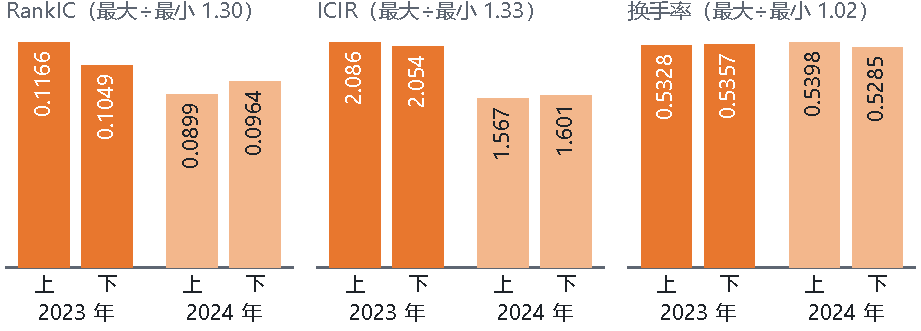
\includegraphics[width=\textwidth]{figures/fig_halfyear_r.pdf}
\source{比赛平台分钟行情，团队本地评测}
\end{figure}

\section{公榜五项轨迹}\label{app:path}

\figref{fig:path} 给出各版本提交公榜时的五项原值，从官方标签核实后的第一个版本开始。五项原值不随其他参评提交变化，不同日期的版本可以直接比较；同一时点比较的增量见附录~\ref{app:increments}。

\begin{figure}[htbp]
\caption{公榜 RankIC 由 0.0898 升至 0.1143，换手率由 0.585 降至 0.508，一次明显回落来自日内细节输入（各版本公榜五项原值）}\label{fig:path}
\centering
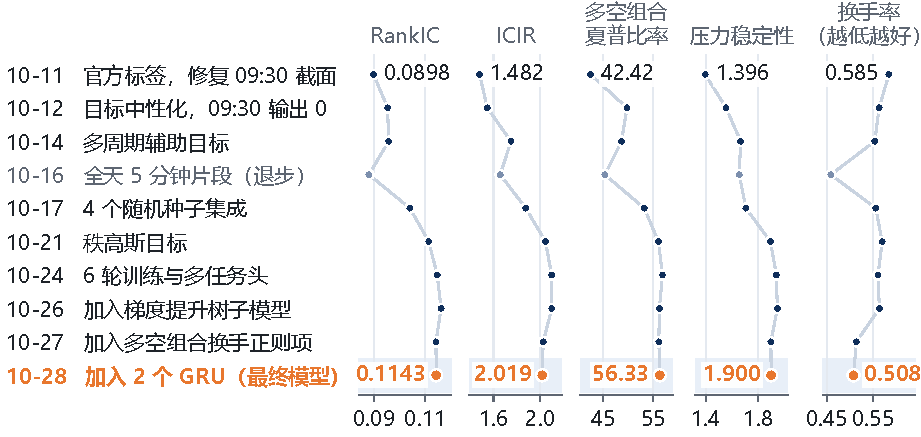
\includegraphics[width=\textwidth]{figures/fig_public_path_r.pdf}
\source{比赛平台公榜，团队整理}
\end{figure}

五项的变化分为三个阶段。第一阶段在核实标签口径、修复 09:30 截面之后，把训练目标改为对行情代理与聚类行业中性化，并让 09:30 截面输出 0，RankIC 由 0.0898 升至 0.0953，压力稳定性由 1.396 升至 1.555。第二阶段加入多周期辅助目标、多随机种子集成与秩高斯目标，RankIC 升至 0.1114，ICIR 由 1.546 升至 2.046；其间全天 5 分钟片段输入使 RankIC 降至 0.0880，这一改动随即撤回。第三阶段加入梯度提升树子模型、多空组合换手正则项与 2 个 GRU 子模型：加入树之后 RankIC 达到全程最高的 0.1162，换手正则项与 GRU 子模型再把换手率由 0.564 降至 0.508，RankIC 保持在 0.114 左右。

\clearpage
\section{术语表}\label{app:terms}

\begin{table}[htbp]
\caption{本文使用的术语}\label{tab:terms}
\centering\tabsetup
\begin{tabularx}{\textwidth}{@{}p{8.2em}>{\raggedright\arraybackslash}X@{}}
\toprule
术语 & 定义\\
\midrule
截面 & 每个交易日 8 个评测时点之一，截面 $t$ 只能使用 $t$ 及之前的数据\\
标签 & 截面之后 30 分钟窗口的收盘价除以同窗口 VWAP 再减 1\\
风格与行业中性化 & 逐截面对 10 个风格因子与 32 个申万一级行业哑变量做含截距的最小二乘回归，取残差\\
多头组合、空头组合 & 每个截面残差排名前 10\%、后 10\% 的等权组合，合称多空名单\\
子模型 & 集成中的单个模型；最终模型有 7 个子模型\\
三尺度网络 & 1 分钟、30 分钟窗口、日线三个时间尺度的编码器加融合头\\
同伴注意力 & 基于走势相似股票的注意力机制：按 60 日收益画像的相似度加权其他股票的表示，自身表示减去这一加权表示\\
秩高斯目标 & 把每个截面的标签平均秩映射为标准正态分位数后作训练目标\\
行情代理风格因子 & 由行情计算的 8 个风格代理与规模平方项，用于训练目标的中性化\\
聚类行业 & 按过去 120 个交易日收益相似度做球面 $k$ 均值聚类得到的 30 类行业，每月更新\\
多周期辅助目标 & 训练目标加上同一交易日之后 2 个截面标签之和的秩高斯目标的 0.5 倍\\
多空组合换手正则项 & 同日相邻截面配对，用 sigmoid 把是否进入多空名单软化为 0～1 的隶属度，惩罚两截面隶属度之差的平方；推理时不使用\\
权重滑动平均 & 训练时对网络参数做衰减系数 0.995 的指数滑动平均，推理加载平均后的参数，与输出平滑无关\\
留出验证设定 & 2020–2022 年训练，2023 年为验证年、2024 年为测试年，两年分别评估\\
留出验证模型 & 与最终模型结构、配方相同，只在留出验证设定下训练的集成\\
单变量线上验证 & 只改动一个变量、只训练到 2022 年、随机种子 42 的单个模型提交公榜，与对照在同一时点比较\\
同一时点比较 & 同一公榜页面上两个提交的五项对照\\
全量训练准入标准 & 进入全量训练前五项增量须满足的阈值\\
\bottomrule
\end{tabularx}
\source{团队整理}
\end{table}

\section{复现与计算资源}\label{app:repro}

训练与推理共用一份冻结的训练脚本，其中包含配置常量、网络结构、数据构建、训练与权重读写。在平台上，脚本直接读取原始行情表与标签表；本地使用同一接口的文件数据后端，本地训练只改写配置常量并加入逐轮验证，调用同一个训练函数。

最终模型的子模型分别在两台机器上训练。一台 Apple M2 Ultra 工作站（192 GB 内存）训练 4 个 Transformer 与梯度提升树，每个 Transformer 耗时 5,176～5,686 秒，峰值内存 60～66 GB，梯度提升树耗时 6,477 秒；一台配 24 GB 显存 GPU、64 GB 内存的工作站训练 2 个 GRU，耗时 1,338 秒与 1,524 秒，峰值内存 51～54 GB。各部分顺序相加约 30,564 秒（约 8.5 小时），这是两种硬件混合的结果，不能据此推算平台重训的耗时。

随机性来源全部固定：子模型 $k$ 使用随机种子 $42+k$，训练单元的打乱顺序、标准化统计量的抽样（20 万个样本）、聚类行业的聚类与梯度提升树的行列抽样都有固定的种子。冻结文件包括训练脚本（2,816 行）、权重文件（30,412,456 字节）与推理 notebook（3,823 字节）。

\end{document}
